\chapter{Design}
\label{chap:design}

This chapter's goal is to describe the overall system design to the reader.
First, the system scopes will be introduced to guide the reader through the system design. After this, the system's architectural design will be presented and major decisions/alternatives are discussed. Then a more detailed vision of the system is given by presenting the domain models of each scope's contexts.

According to \cite{DIAS2022100529}, \gls{IoT} solutions, on a high-level, are commonly composed by three tiers:

\begin{itemize}
   \item Cloud Tier: Servers, Applications and Data Centers;
   \item Fog Tier: Routes and Gateways;
   \item Edge Tier: Embedded Systems, sensors and actuators (things).
\end{itemize}

This chapter focus only on the Cloud Tier, the other tiers are out of scope since the author had no relevant involvement in their development.

To ease the interpretation of the solution's architectural design it was divided according to two subjects, scopes and concept/concern/capability.
Scopes are derived from the major system responsibilities of the solution as a whole, concept/concern/capability are derived from the major functionalities or business cases that the project has to answer.

\section{System Scopes}
\label{sec:design:system_scopes}

The solution designed can be divided in three main scopes as disclosed in Figure~\ref{fig:design:system_scopes:scopes}.

\begin{figure}[H]
    \centering
   \resizebox{\columnwidth}{!}
   {
      \input{assets/diagrams/design/scopes.latex}
   }
   \caption[System Scopes]{System Scopes}
   \label{fig:design:system_scopes:scopes}
\end{figure}

The \textbf{Sensae Console} is composed by two scopes, \textbf{Configuration Scope} and \textbf{Data Flow Scope}. These scopes are static and always available in any installation. They answer core/common functionalities of any \gls{IoT}-based service.

The \textbf{External Services Scope} is where actual business cases concerns are tackled. This scope is dynamic, meaning that an installation can have different types of external services depending on the costumer needs. The requested \gls{PoC}s belong to this scope.

The \textbf{Configuration Scope} refers to the configuration and visualization of internal processes/contexts. Processes such as: (i) data decoders, (ii) data mappers (iii) device inventory, (iv) warning rule scenarios definition and (v) device ownership - related to the \textbf{Data Flow Scope}. It is also possible to manage users' access and permissions in this scope.

The \textbf{Data Flow Scope} acts as a pipeline where raw data, device uplinks, goes through various stages till it is sanitized and ready to be supplied to the \textbf{External Services Scope}. The \textbf{Data Flow Scope} is where internal processes occur, such as: (i) data transformation, (ii) data enrichment, (iii) data validation, (iv) data ownership clarification and (v) alerts dispatching. It behaves according to what is defined in the \textbf{Configuration Scope}.

The \textbf{External Services Scope} is comprised of services that present and act according to the sanitized data and alerts that were supplied to them. These services applicability range from (i) smart irrigation, (ii) fleet management, (iii) fire detention, (iv) physical security access monitoring, (v) air quality monitoring and anything else deemed interesting. The services currently developed are smart irrigation, fleet management and notification management. These will be addressed throughout this and the \nameref{chap:implementation} chapter.

\subsection{Configuration Scope}
\label{subsec:design:system_scopes:configuration_scope}

The \textbf{Configuration Scope} is responsible for managing the following contexts:

\begin{itemize}
   \item \textbf{Data Processor}: manages simple data mappers;
   \item \textbf{Data Decoder}: manages scripts to transform data;
   \item \textbf{Device Management}: manages device information such as name, metadata, static data and other notions;
   \item \textbf{Identity Management}: manages device ownership and users permissions;
   \item \textbf{Rule Management}: manages scripts that consume device data and produce alerts.
\end{itemize}

This contexts can be directly linked to the functional requirements described in the Section related to the~\ref{subsubsec:requirements:functional:sensae:manager} role.

Each context allows an authorized user to manage its resources, e.g. the data processor context manages the creation, deletion and renovation of data mappers.

This operations require various verification's, alter the system internal state and are therefore prolonged operations.

\subsection{Data Flow Scope}
\label{subsec:design:system_scopes:data_flow_scope}

The \textbf{Data Flow Scope} is responsible for processing incoming data according to what is defined in the \textbf{Configuration Scope}. Both scopes share the same contexts.

This scope also contains three independent units, that aren't controlled by the \textbf{Configuration Scope}:

\begin{itemize}
   \item Data Gateway: responsible for providing a bridge between the \gls{IoT} middlewares and the \textbf{Sensae Console};
   \item Data Validator: responsible for filtering device measures based on static rules, e.g. battery percentage reported has to be in between 0 and 100.
   \item Data Store: responsible for persisting data captured in a defined state.
\end{itemize}

This scope applies changes to the device measures that flow though the system. This changes are stateless and don't change the overall state of the internal system state.

This scope was decoupled from the \textbf{Configuration Scope} even though they both work with the same contexts. The decision was taken based on the pretext that despite the similarities in context the operation/business responsibilities of this two scopes were conflicting.

The \textbf{Configuration Scope} requires scarce but heavy computations that alter the internal system state while the \textbf{Data Flow Scope} requires plentiful but light computations that don't alter the internal system state as summarized in the Table~\ref{tab:design:system_scopes:data_flow_scope:comparison}.

\begin{table}[!ht]
   \caption[Comparison of Operations in Data Flow and Configuration Scopes]{Comparison of Operations in Data Flow and Configuration Scopes}
   \label{tab:design:system_scopes:data_flow_scope:comparison}
   \centering
   \begin{tabular}{@{}lllll@{}}
   \toprule
   \textbf{Comparison of Operations} & \textbf{Configuration Scope} & \textbf{Data Flow Scope} \\ \midrule
       Alter internal system state & yes & no \\ \hline
       Alter sensor data & no & yes \\ \hline
       Required computation power/time & high & low \\ \hline
       Frequency of usage & low & high \\ \hline
   \end{tabular}
\end{table}

Due to this discrepancy it's expected for each scope to have different requirements regarding horizontal scaling. With the addition of more devices to the platform, and subsequently higher ingress volume, \textbf{Data Flow Scope} will need to scale. Since the \textbf{Configuration Scope} is intended mostly for the manager of the platform, a small user pool, the need to scale is smaller.

\subsection{External Services Scope}
\label{subsec:design:system_scopes:service_scope}

The \textbf{External Services Scope} is responsible for presenting \gls{IoT} business cases to end users. This scope is detached from the \textbf{Sensae Console} due to its dynamic nature. The services that belong to this scope are analogous to plugins.

The scope is comprised of services that consume data and publish commands to \textbf{Data Flow Scope}. Currently, as a \gls{MVP} the implemented business cases are:

\begin{itemize}
   \item \textbf{Fleet Management}: basic service to monitor a fleet of cars regarding their location;
   \item \textbf{Smart Irrigation}: service to automate and monitor the irrigation of zones based on sensor readings;
   \item \textbf{Notification Management}: service to view and manage the delivery of triggered alerts.
\end{itemize}

Each service is bounded to what type of data receives and sends back to the \textbf{Data Flow Scope} as later detailed in the \nameref{subsec:implementation:description:services} section. The type of data each service handles is enforces by the concepts discussed in Sections~\ref{subsec:design:domain:taxonomy} and \ref{subsec:design:domain:shared_model}.

Just like plugins, services in this scope are validate and attached to the final deployment by the entity that manages that specific instance. When working in a multi-tenant, shared instance, custom external services can't be properly verified and therefore their usage is denied.

\section{Architectural Design}
\label{sec:design:architecture}

In order to describe the system in detail at the architectural level, an approach based on the combination of two models, C4 (\cite{c4model-site}) and 4+1  will be followed.

The 4+1 View Model (\cite{4plus1model}), proposes the description of the system through complementary views thus allowing to separately analyze the requirements of various software stakeholders, such as users, system administrators, project managers, architects, and programmers.

The five views are thus defined as follows:
\begin{itemize}
   \item \textbf{Logical view}: relative to the aspects of the software aimed at responding to business challenges;
   \item \textbf{Process view}: relative to the process flow or interactions within the system;
   \item \textbf{Implementation View}: relative to the organization of the software in its development environment;
   \item \textbf{Physical view}: relative to the mapping of the various components of the software in hardware, i.e. where the software is executed;
   \item \textbf{Scenario view}: related to the association of business processes with actors capable of triggering them.
\end{itemize}

The C4 Model (\cite{c4model-site}, \cite{c4model}) advocates describing software through four levels of abstraction:
(i) system, (ii) container, (iii) component, (iv) code. Each level adopts a finer granularity than the level that precedes it, thus giving access to more details of a smaller portion of the system.
These levels can be likened to maps, e.g. the system view corresponds to the globe, the container corresponds to the map of each continent, the component view corresponds to the map of each of each country, and the code view to the map of roads and neighborhoods in each city.

Different levels allow you to tell different stories to different audiences.

The levels are defined as follows:

\begin{itemize}
   \item \textbf{Level 1}: Description (context) of the system as a whole;
   \item \textbf{Level 2}: Description of system containers;
   \item \textbf{Level 3}: Description of components of the containers;
   \item \textbf{Level 4}: Description of the code or smaller parts of the components.
\end{itemize}

These two models can be said to expand along distinct axes, with the C4 Model presenting the system with different levels of detail and the 4+1 View Model presenting the system from different perspectives. By combining the two models it becomes possible to represent the system from several perspectives, each with various levels of detail.
To visually model/represent the ideas designed and alternatives considered, the \gls{UML} was used.

In the following sections only combinations of perspectives and level deemed relevant for the design of the solution are presented.

The C4 level 4, code, will not be exhibited.

\subsection{C4 Level 1 - Context}
\label{subsec:design:architecture:context}

The context level aims at introducing the system as a whole. The external systems and users that communicate/interact with the system, \textbf{Sensae Console}, are demonstrated.
Throughout this section the relevant C4 views of level 1 (context level) are presented.

\subsubsection{Context Level - Logical View}
\label{subsubsec:design:architecture:context:logical}

The logical view of the system is introduced here, complete but not detailed, in order to answer the use cases and requirements discussed in Chapter~\ref{chap:requirements}. This takes into account the interactions of \textbf{Sensae Console} and \textbf{External Services} with foreign systems and its interaction with the various actors of the system (Figure~\ref{fig:design:architecture:context:logical:diagram}) as required by Section~\ref{subsec:requirements:non_functional:design}.

\begin{figure}[H]
   \centering
   \resizebox{0.8\columnwidth}{!}
   {
      \input{assets/diagrams/design/architectural/level1/logical-view.latex}
   }
   \caption[Context Level - Logical View Diagram]{Context Level - Logical View Diagram}
   \label{fig:design:architecture:context:logical:diagram}
\end{figure}

The \textbf{External Services} are represented as an independent system that consumes the \textbf{Sensae Console} \gls{API}. This \gls{API} is responsible for streaming information such as device measures, device commands, alerts and internal state asynchronously. These concept's semantics and structure are enforced by a library, \textit{iot-core}, also developed and discussed in Section~\ref{subsec:design:domain:shared_model}.

Both of the \textit{systems} provide an \gls{API} for automated management/control and a \gls{UI} for ease of use and data visualization.

As mentioned before in Section~\ref{subsubsec:requirements:functional:services:fire} there is a need to integrate the final product with an Email and SMS dispatch service.

The reason that lead to the use of external authentication/identity services, as required in Section~\ref{subsec:requirements:non_functional:interface}, is further discussed in the Section~\ref{subsec:design:alternatives:auth}.

\subsubsection{Context Level - Physical View}
\label{subsubsec:design:architecture:context:physical}

Next is the physical view (Figure~\ref{fig:design:architecture:context:physical:diagram}), intended to familiarize the reader with the environment where the solution runs.

\begin{figure}[H]
   \centering
   \resizebox{\columnwidth}{!}
   {
      \input{assets/diagrams/design/architectural/level1/physical-view.latex}
   }
   \caption[Context Level - Physical View Diagram]{Context Level - Physical View Diagram}
   \label{fig:design:architecture:context:physical:diagram}
\end{figure}

The Identity Providers currently in use by the solution are \cite{googleid} and \cite{azureid} both of this platforms provide an OpenID Connect \gls{API}.

The SMS dispatching service is the \textit{Twilio Platform}. The Email dispatching service is the \textit{Google Email Platform}. And finally, the only \gls{IoT} Middleware in use currently is \cite{helium}.

\subsubsection{Context Level - Synopsis}
\label{subsubsec:design:architecture:context:synopsis}

The context level introduces the reader to the bigger picture of \textbf{Sensae Console}, but it contains little to no information about how the system functions internally, the Section~\ref{subsec:design:architecture:containers} will dive into this subject.

The process view was not represented since at this level the interactions between the system, actors and external systems, are too abstract to be relevant for the reader.

The implementation view was also not represented since the \textbf{Sensae Console} and \textbf{External Services} were developed as a single project.

\subsection{C4 Level 2 - Containers}
\label{subsec:design:architecture:containers}

The C4 level 2 introduces the reader to the various containers that compose the system. In this section all relevant views will be presented according to the alternative in use or idealized for the system. In the Section~\ref{sec:design:alternatives} other alternatives are discussed.

The description of this level of abstraction begins with a logical view of the containers that compose the system.

\subsubsection{Container Level - Logical View NEW}

In order to support the functional requirements identified (Section~\ref{sec:requirements:functional}), and knowing that \textbf{Sensae Console} will serve multiple users with different levels of access to the managed information, the various business concepts were segregated from the user interaction. The business management also had to be separated from the  data pipeline, knowing that \textbf{Sensae Console} will process a high volume of device measures.

Considering the need to persist and provide the information collected, the system integrates databases, which are not developed, but only configured and operated - using a \gls{DBMS}.

The system also uses one (or more) message brokers, \cite{broker}, that will be configured but not developed.

In order to ease the analysis of the system the following diagram, Figure~\ref{fig:design:architecture:containers:logical:complete}, presents a complete view of \textbf{Sensae Console} where each concept/concern/capability represents a group of containers that focus on the same concern. These groups are them explored in detail.

\begin{sidewaysfigure}
      \centering
   \resizebox{0.8\columnwidth}{!}
   {
      \input{assets/diagrams/design/architectural/level2/logical/contexts-v2.latex}
   }
   \caption[Sensae Console - Container Level - Logical View Diagram]{Sensae Console - Container Level - Logical View Diagram}
      \label{fig:design:architecture:containers:logical:complete}
\end{sidewaysfigure}

As seen in the diagram:

\begin{itemize}
   \item Each concept/concern/capability exposes a \gls{UI} and an \gls{API}, these are aggregated in the \gls{UI} Aggregator container that then exposes everything as a single \gls{UI} and \gls{API} for management;
   \item The Device Management concept/concern/capability consumes the \gls{IoT} Middleware API since it is responsible for sending downlinks to devices;
   \item The Message Broker exposes an \gls{API}, this is the \gls{API} that the \textbf{External Services} consume to access the information that flow in \textbf{Sensae Console};
   \item The Identity Management concept/concern/capability consumes the Identity Provider's OpenID Connect API to handle User Authentication;
   \item The Message Broker is responsible for routing messages through the system and ensuring that the various containers communicate;
   \item The Data Store Backend and Data Store Database are responsible for store data in a specific format, defined at startup;
   \item The Data Relayer and Data Gateway are responsible for exposing an \gls{API} for data ingestion and publish the ingested data in the system through the Message Broker;
   \item The Data Validator applies simple filters to incoming data, for example, measures that report a soil moisture of 120\% as marked as incorrect.
\end{itemize}

Each concept/concern/capability is composed by containers that belong to the \textbf{Configuration} and \textbf{Data Flow} Scopes (represented in yellow in the following diagrams).

The Configuration Scope of each concept/concern/capability is composed by a three layers architecture, as per \cite{3tier}:

\begin{itemize}
   \item \textbf{Presentation Layer}: the user interface and communication layer of the application where the user interacts with the system;
   \item \textbf{Application Layer}: the business layer of the application where information from the \textbf{Presentation Layer} is processed and sent to the \textbf{Data Layer};
   \item \textbf{Data Layer}: the infrastructure layer of the application where data is stored and requested as needed.
\end{itemize}

The Data Flow Scope is usually composed by a single container that only consumes the Message Broker \gls{API}.

As a brief description of some of the similar characteristics of all concept/concern/capability:

\begin{itemize}
   \item The frontend container corresponds to the \textbf{Presentation Layer} and exposes an \gls{UI};
   \item The backend container corresponds to the \textbf{Application Layer} and communication with the Data Flow container(s) exclusively through the \textbf{Message Broker}. The Backend publishes issues related to the concept/concern/capability configuration that the Data Flow Container consumes. The Data Flow container publishes metrics related to what resources are being used that are then consumed by the Backend;
   \item The communication exchanged between Backend and Data Flow containers is parameterized according to the Section~\ref{subsubsec:design:domain:shared_model:routing} and is preformed in the Internal Topic;
   \item The backend container also exposes an \gls{API} that is consumed by the frontend and optionally by properly authenticated external systems;
   \item The database container correspond to the \textbf{Data Layer}.
\end{itemize}

The Data Processor concept/concern/capability group is presented in Figure~\ref{fig:design:architecture:containers:logical:processor}.

\begin{figure}[H]
   \centering
   \resizebox{\columnwidth}{!}
       {
       \input{assets/diagrams/design/architectural/level2/logical/data-processor-context.latex}
       }
   \caption[Data Processor - Container Level - Logical View Diagram]{Data Processor - Container Level - Logical View Diagram}
   \label{fig:design:architecture:containers:logical:processor}
\end{figure}

This concept/concern/capability is responsible for transforming the data received in a format and semantic that can be understood by the system, it is explored in detail in Section~\ref{subsubsec:design:domain:bounded_contexts:processor}. The Data Processor Data Flow publishes metrics to the Message Broker regarding the time each Data Processor was used so that the Backend can then report this usages.

The Data Decoder concept/concern/capability group is presented in Figure~\ref{fig:design:architecture:containers:logical:decoder}.

\begin{figure}[H]
   \centering
   \resizebox{\columnwidth}{!}
       {
       \input{assets/diagrams/design/architectural/level2/logical/data-decoder-context.latex}
       }
   \caption[Data Decoder - Container Level - Logical View Diagram]{Data Decoder - Container Level - Logical View Diagram}
   \label{fig:design:architecture:containers:logical:decoder}
\end{figure}

This concept/concern/capability is also responsible for transforming the data received in a format and semantic that can be understood by the system. In contrast with the Data Processor, it provides a more flexible but complex way of manipulating data, it is explored in detail in Section~\ref{subsubsec:design:domain:bounded_contexts:decoder}. The Data Decoder Data Flow publishes metrics to the Message Broker regarding the time each Data Decoder was used so that the Backend can then report this usages.

The Device Management concept/concern/capability group is presented in Figure~\ref{fig:design:architecture:containers:logical:device}.

\begin{figure}[H]
   \centering
   \resizebox{\columnwidth}{!}
       {
       \input{assets/diagrams/design/architectural/level2/logical/device-management-context.latex}
       }
   \caption[Device Management - Container Level - Logical View Diagram]{Device Management - Container Level - Logical View Diagram}
   \label{fig:design:architecture:containers:logical:device}
\end{figure}

This concept/concern/capability is responsible for maintaining a registry of the devices in use by the platform.

The Device Management Data Flow enriching the measures collected with more information regarding the device that sent them. The Device Commander consumes an \gls{IoT} Middleware REST \gls{API} to dispatch downlinks to devices. This downlinks contain commands that control the behavior of the implied actuator.
This concept/concern/capability is explored in Section~\ref{subsubsec:design:domain:bounded_contexts:device}. The Data Flow containers publishes metrics to the Message Broker regarding the time each device was used so that the Backend can then report this usages.

The Rule Management concept/concern/capability group is presented in Figure~\ref{fig:design:architecture:containers:logical:rule}.

\begin{figure}[H]
   \centering
   \resizebox{\columnwidth}{!}
       {
       \input{assets/diagrams/design/architectural/level2/logical/rule-management-context.latex}
       }
   \caption[Rule Management - Container Level - Logical View Diagram]{Rule Management - Container Level - Logical View Diagram}
   \label{fig:design:architecture:containers:logical:rule}
\end{figure}

This concept/concern/capability is responsible for managing rule scenarios that produce alerts based on the captured device measures.

The Alert Dispatcher is responsible for publishing alerts based on the rule scenarios published by the Rule Management Backend. The Rule Management Backend ensures that the rules submitted are valid. This concept/concern/capability is explored in Section~\ref{subsubsec:design:domain:bounded_contexts:rule}. This data flow container does not publishes any metrics, its interactions are better described with the help of sequence diagrams available in Figures~\ref{fig:design:architecture:container:process:diagram:init} and \ref{fig:design:architecture:component:process:diagram:rule}.

The Identity Management concept/concern/capability group is presented in Figure~\ref{fig:design:architecture:containers:logical:identity}.

\begin{figure}[H]
   \centering
   \resizebox{\columnwidth}{!}
       {
       \input{assets/diagrams/design/architectural/level2/logical/identity-management-context.latex}
       }
   \caption[Identity Management - Container Level - Logical View Diagram]{Identity Management - Container Level - Logical View Diagram}
   \label{fig:design:architecture:containers:logical:identity}
\end{figure}

This concept/concern/capability is responsible for managing devices ownership, user identity and organization's details. The backend and frontend containers communicate with an identity provider via OpenID Connect to verify the user identity. The Device Ownership Backend enriches the data measures and alerts with information regarding the organizations that own the device responsible for sending the measures or that lead to the dispatch of an alert. This concept/concern/capability is explored in Section~\ref{subsubsec:design:domain:bounded_contexts:identity}. This data flow container publishes metrics to the Message Broker regarding the time each organization information was used.

As the diagrams above presented, all communication between backend containers of both scopes is guaranteed by the Message Broker. This Message Broker exposes its \gls{API} so that External Services can consume all information and act according to it. The next diagrams present the three External Services that were developed.

Some of the similarities shared between the architecture of all services are:

\begin{itemize}
   \item All contain a backend that exposes an \gls{API};
   \item All contain a frontend that exposes a \gls{UI};
   \item All contain at least a database that exposes an \gls{API} consumed solely by the backend;
   \item Any communication with \textbf{Sensae Console} is preformed by consuming the Message Broker's \gls{API};
   \item All follow the idea behind the separation of responsibilities seen in a three layer architecture;
\end{itemize}

The Fleet Management service is presented in Figure~\ref{fig:design:architecture:containers:logical:fleet}.

\begin{figure}[H]
   \centering
   \resizebox{\columnwidth}{!}
       {
       \input{assets/diagrams/design/architectural/level2/logical/fleet-management-context.latex}
       }
   \caption[Fleet Management - Container Level - Logical View Diagram]{Fleet Management - Container Level - Logical View Diagram}
   \label{fig:design:architecture:containers:logical:fleet}
\end{figure}

This service is composed by a simple three layers architecture. The details related to this service are discussed in Section~\ref{subsubsec:design:domain:bounded_contexts:fleet}.

The Notification Management service is presented in Figure~\ref{fig:design:architecture:containers:logical:noti}.

\begin{figure}[H]
   \centering
   \resizebox{\columnwidth}{!}
       {
       \input{assets/diagrams/design/architectural/level2/logical/notification-management-context.latex}
       }
   \caption[Notification Management - Container Level - Logical View Diagram]{Notification Management - Container Level - Logical View Diagram}
   \label{fig:design:architecture:containers:logical:noti}
\end{figure}

This service is composed by a simple three layers architecture and has a separated container responsible for dispatching SMS and emails, the Notification Dispatcher Backend container. Information regarding the type of alerts each user is interested in are exchanged between the Backend and Dispatcher containers through the Message Broker. The details related to this service are discussed in Section~\ref{subsubsec:design:domain:bounded_contexts:fleet}.

Finally, the Smart Irrigation Management service is presented in Figure~\ref{fig:design:architecture:containers:logical:irrigation}.

\begin{figure}[H]
   \centering
   \resizebox{\columnwidth}{!}
       {
       \input{assets/diagrams/design/architectural/level2/logical/smart-irrigation-context.latex}
       }
   \caption[Smart Irrigation - Container Level - Logical View Diagram]{Smart Irrigation - Container Level - Logical View Diagram}
   \label{fig:design:architecture:containers:logical:irrigation}
\end{figure}

This service is composed by a three layers architecture, the \textbf{Data Layer} is divided in two databases, one responsible for storing device measures and another responsible for storing information regarding the Irrigation Zones and device information. The details related to this service are discussed in Section~\ref{subsubsec:design:domain:bounded_contexts:irrigation}.

As a final note, even though it isn't required, the \textbf{UI Aggregator} can be configured to consume the \gls{UI} and \gls{API} belonging to each External Services. By doing so, the complete solution, \gls{UI} and \gls{API} can be presented under a single \gls{FQDN}. This view can be seen in Appendix~\ref{AppendixB}.

In the following section the internal communication of the system is clarified.

\subsubsection{Container Level - Logical View - OLD}
\label{subsubsec:design:architecture:container:logical}

In order to support the functional requirements identified (Section~\ref{sec:requirements:functional}), and knowing that \textbf{Sensae Console} will serve multiple users with different levels of access to the managed information, the various business concepts were segregated from the user interaction. The business management also had to be separated from the  data pipeline, knowing that \textbf{Sensae Console} will process a high volume of device measures.

Considering the need to persist and provide the information collected, the system integrates databases, which are not developed, but only configured and operated - using a \gls{DBMS}.

The system also uses one (or more) message brokers, \cite{broker}, that will be configured but not developed.

In order to ease the analysis of the system the following diagrams will be divided by scopes, mentioned in \ref{sec:design:system_scopes}. In the Appendix~\ref{AppendixB} a complete logical view is provided.

The logical view of the \textbf{Configuration Scope} is represented in Figure~\ref{fig:design:architecture:container:logical:diagram:configuration}. This scope is composed by the processes discussed in \ref{subsec:design:system_scopes:configuration_scope}. Each process is composed by a three layer architecture, as per \cite{3tier}:

\begin{itemize}
   \item \textbf{Presentation Layer}: the user interface and communication layer of the application where the user interacts with the system;
   \item \textbf{Application Layer}: the business layer of the application where information from the \textbf{Presentation Layer} is processed and sent to the \textbf{Data Layer};
   \item \textbf{Data Layer}: the infrastructure layer of the application where data is stored and requested as needed.
\end{itemize}

This scope was also divided into micro services - \cite{newman2021building} - \textit{'small, autonomous services that work together'}. Each bounded context/business process - (i) Data Processor, (ii) Data Decoder, (iii) Device Management, (iv) Identity Management, (v) Rule Management - is mapped to the three layer architecture mention before.

\begin{landscape}
   \begin{figure}[H]
      \centering
   \resizebox{\columnwidth}{!}
   {
      \input{assets/diagrams/design/architectural/level2/logical/configuration.latex}
   }
   \caption[Container Level - Configuration Scope - Logical View Diagram]{Container Level - Configuration Scope - Logical View Diagram}
      \label{fig:design:architecture:container:logical:diagram:configuration}
   \end{figure}
\end{landscape}

As a brief description:

\begin{itemize}
   \item Frontend containers correspond to the \textbf{Presentation Layer} and are provided to the user through \textbf{UI Aggregator};
   \item Backend containers correspond to the \textbf{Application Layer} and communication with each other through \textbf{Message Broker};
   \item Database containers correspond to the \textbf{Data Layer}.
\end{itemize}

Next, the logical view of the \textbf{Data Flow} is represented in Figure~\ref{fig:design:architecture:container:logical:diagram:data_flow}. This scope is composed by the processes discussed in \ref{subsec:design:system_scopes:data_flow_scope}. In parallel with the \textbf{Configuration Scope} this scope is also divided into multiple micro services in order for them to better scale once needed. This scope is also built based on a \textit{Reactive architecture} as described in \cite{reactivemanifesto} and \cite{reactivesystem}.

\begin{figure}[H]
   \centering
   \resizebox{\columnwidth}{!}
   {
      \input{assets/diagrams/design/architectural/level2/logical/data-flow.latex}
   }
   \caption[Container Level - Data Flow Scope - Logical View Diagram]{Container Level - Data Flow Scope - Logical View Diagram}
   \label{fig:design:architecture:container:logical:diagram:data_flow}
\end{figure}

Most containers presented here collect specific information from a single backend in the \textbf{Configuration Scope} through the \textit{Internal} Topic:

\begin{itemize}
   \item \textbf{Data Processor Flow Backend}: Collects information related to the \textbf{Data Processor} context - published by \textbf{Data Processor Backend} - and nothing else;
   \item \textbf{Data Decoder Flow Backend}: Collects information related to the \textbf{Data Decoder} context - published by \textbf{Data Decoder Backend} - and nothing else;
   \item \textbf{Device Ownership Backend}: Collects information related to the \textbf{Identity Management} context (more specifically device ownership) - published by \textbf{Identity Management Backend} - and nothing else;
   \item \textbf{Device Management Flow Backend}: Collects information related to the \textbf{Device Management} context - published by \textbf{Device Management Backend} - and nothing else;
   \item \textbf{Alert Dispatcher Backend}: Collects information related to the \textbf{Rule Management} context - published by \textbf{Rule Management Backend} - and nothing else;
   \item \textbf{Device Command Backend}: Collects information related to the \textbf{Device Management} context - published by \textbf{Device Management Backend} - and nothing else;
   \item The remaining containers don't subscribe to any type of information from the \textbf{Configuration Scope}.
\end{itemize}

Finally the \textbf{External Services Scope} is represented in Figure~\ref{fig:design:architecture:container:logical:diagram:service}. This scope is composed by the processes discussed in \ref{subsec:design:system_scopes:service_scope}.

\begin{figure}[H]
   \centering
   \resizebox{\columnwidth}{!}
   {
      \input{assets/diagrams/design/architectural/level2/logical/service.latex}
   }
   \caption[Container Level - External Services Scope - Logical View Diagram]{Container Level - External Services Scope - Logical View Diagram}
   \label{fig:design:architecture:container:logical:diagram:service}
\end{figure}

Once again the ideas behind this scope architecture are the same discussed in the \textbf{Configuration Scope} apart from two particular points:

\begin{itemize}
   \item \textbf{Smart Irrigation Data Database/Business Database}: As explained in the domain presented in \ref{subsubsec:design:domain:bounded_contexts:irrigation}, since there are two distinct types of information to store and manage it was decided to use different technologies for each type;
   \item \textbf{Notification Management/Dispatcher Backend}: It was also decided to split the delivery of notifications (by email and SMS) from their management.
\end{itemize}

Lastly, as we can seen some containers are present in more than one scope. These containers, and their responsibilities are:

\begin{itemize}
   \item \textbf{Message Broker}: Container responsible for routing messages/events sent by backend containers. This communication is explored in the section, \nameref{subsubsec:design:architecture:container:process};
   \item \textbf{UI Aggregator}: Container responsible for aggregating all frontends in a single \gls{UI}.
\end{itemize}

In the following section the internal communication of the system is clarified.

\subsubsection{Container Level - Process View}
\label{subsubsec:design:architecture:container:process}

In this section several use cases (according to some functional requirements identified in Section~\ref{sec:requirements:functional}) are presented through sequence diagrams, in order to introduce the reader to the interactions that occur between the various containers of the \textbf{Sensae Console}.

The routing keys used for communication between backend containers can be extrapolated from the model described in the Section~\ref{subsubsec:design:domain:shared_model:routing}.

This section is composed by five sets of important functionalities to discuss at this level of abstraction: (i) system/container initialization (ii) data pipeline operation, (iii) data pipeline configuration, (iv) user authentication/authorization, (v) service usage.

The system/container initialization, presented in Figure~\ref{fig:design:architecture:container:process:diagram:init}, refers to the interval of time since a container is launched till it is ready to process requests or events.

\begin{figure}[H]
   \centering
   \resizebox{\columnwidth}{!}
   {
      \input{assets/diagrams/design/architectural/level2/process/container-init.latex}
   }
   \caption[Container Level - System/Container Initialization - Process View Diagram]{Container Level - System/Container Initialization - Process View Diagram}
   \label{fig:design:architecture:container:process:diagram:init}
\end{figure}

Not all containers are displayed in this diagram for brevity reasons.
The system relies heavily in the Pub/Sub (\cite{pubsub}) pattern to communicate internally via a message broker. In this scenario the first step in a container life cycle is to subscribe to the information that it needs as presented in the diagram above.

Certain containers need the entire state related to their \textit{ContextType} to function. So, after subscribing to the needed information, they notify the system that they have entered an \textit{init state} for a specific context. This triggers the creation of new events to help that container to reach a \textit{ready state}. An example of this interaction is presented in the following diagram, Figure~\ref{fig:design:architecture:container:process:diagram:ready}, this only occurs in the Internal Topic.

\begin{figure}[H]
   \centering
   \resizebox{\columnwidth}{!}
   {
      \input{assets/diagrams/design/architectural/level2/process/container-ready.latex}
   }
   \caption[Container Level - System/Container Initialization - Part 2 - Process View Diagram]{Container Level - System/Container Initialization - Part 2 - Process View Diagram}
   \label{fig:design:architecture:container:process:diagram:ready}
\end{figure}

Apart from the Alert Dispatcher Backend, all containers in the \textbf{Data Flow Scope} benefit from a stateless process and can function with just a portion of a single \textit{ContextType} state or no state at all.

To dive into this, some common data pipeline operations, related to the Data Flow Scope, are presented next. This operations are intended to behave in a \textit{reactive} manner (\cite{reactivemanifesto}) and are therefore non-blocking. The idea behind the Data Flow Scope is analog to a data pipeline. This scope operates mostly on Data Units, transforming, filtering and enriching this data.

The following diagram in Figure~\ref{fig:design:architecture:container:process:diagram:flow} presents a high level view of the flow that a Data Unit takes through the system in the Data topic. This diagram does not account for what happens to invalid Data Units and the interactions with the message broker are hidden for brevity reasons even though it is used by all containers to publish messages.

\begin{figure}[H]
   \centering
   \resizebox{\columnwidth}{!}
   {
      \input{assets/diagrams/design/architectural/level2/process/data-flow-scope.latex}
   }
   \caption[Container Level - Data Flow - Diagram]{Container Level - Data Flow - Diagram}
   \label{fig:design:architecture:container:process:diagram:flow}
\end{figure}

Most of these containers have just a portion of their context state and may be unable to preform the needed operation on some Data Units. The following diagrams, Figure~\ref{fig:design:architecture:container:process:diagram:decoder:1} and Figure~\ref{fig:design:architecture:container:process:diagram:decoder:2}, addresses how state is managed in Data Decoder Flow Backend and most \textbf{Data Flow Scope} containers.

\begin{figure}[H]
   \centering
   \resizebox{\columnwidth}{!}
   {
      \input{assets/diagrams/design/architectural/level2/process/data-decoder-flow-1.latex}
   }
   \caption[Container Level - Data Decoder Operation part 1 - Process View Diagram]{Container Level - Data Decoder Operation Part 1 - Process View Diagram}
   \label{fig:design:architecture:container:process:diagram:decoder:1}
\end{figure}

As we can see, the Data Decoder Flow Backend, upon receiving a Data Unit, can preform two operations, whether or not the script is available: decode the Data Unit and notify that the script was used or store the Data Unit and notify that a script for an unknown device type is needed.

The next diagram describes what happens when a message with a decoder is published (using the \textit{OperationType} Info mentioned in Section~\ref{subsubsec:design:domain:shared_model:routing}).

\begin{figure}[H]
   \centering
   \resizebox{\columnwidth}{!}
   {
      \input{assets/diagrams/design/architectural/level2/process/data-decoder-flow-2.latex}
   }
   \caption[Container Level - Data Decoder Operation Part 2 - Process View Diagram]{Container Level - Data Decoder Operation Part 2 - Process View Diagram}
   \label{fig:design:architecture:container:process:diagram:decoder:2}
\end{figure}

As we can see Data Decoder Flow Backend, upon receiving an info regarding a data decoder, searches for unhandled Data Units and processes them.
To minimize the memory in use, a data decoder has to be continually used in order for it to remain in cache. As seen in step \textbf{2.2}, if \textit{X} hours pass since the last time a decoder was used it is evicted from the container internal state.

The operations described here for the Data Decoder Flow Backend are replicated in the following contexts/containers:

\begin{itemize}
   \item \textbf{Data Processor Context}: Data Processor Flow Backend;
   \item \textbf{Device Management Context}: Device Management Flow Backend and Device Commander Backend;
   \item \textbf{Identity Management Context}: Device Ownership.
\end{itemize}

As described before, containers that belong to the \textbf{Data Flow Scope} operate according to what the \textbf{Configuration Scope} defined.

The next diagrams, in Figure~\ref{fig:design:architecture:container:process:diagram:processor} and Figure~\ref{fig:design:architecture:container:process:diagram:device} present some of the common operations that happen in that scope.

\begin{figure}[H]
   \centering
   \resizebox{\columnwidth}{!}
   {
      \input{assets/diagrams/design/architectural/level2/process/consult-data-processor.latex}
   }
   \caption[Container Level - Consult Data Processors - Process View Diagram]{Container Level - Consult Data Processors - Process View Diagram}
   \label{fig:design:architecture:container:process:diagram:processor}
\end{figure}

The diagram presented above represents a simple consult of data mappers, as we can see, only the Data Processor Context in the Configuration Scope is invoked. When a change to the state is made in any Context of the Configuration Scope, events are published. The next diagram, Figure~\ref{fig:design:architecture:container:process:diagram:device} displays an example of this occurrence.

\begin{figure}[H]
   \centering
   \resizebox{\columnwidth}{!}
   {
      \input{assets/diagrams/design/architectural/level2/process/edit-device-management.latex}
   }
   \caption[Container Level - Edit Device Information - Process View Diagram]{Container Level - Edit Device Information - Process View Diagram}
   \label{fig:design:architecture:container:process:diagram:device}
\end{figure}

In this use case a device information is changed. Since this operation changes the internal state of the device management context, an event is published in the Internal Topic.

As an example of this specific event, according to the Section~\ref{subsubsec:design:domain:shared_model:routing}, uses the following \textit{Routing Keys}:

\begin{itemize}
   \item \textbf{Protocol Version}: the version of \textit{iot-core} currently in use by Device Management Backend;
   \item \textbf{Container Type}: Device Management Backend;
   \item \textbf{Topic Type}: Internal;
   \item \textbf{Operation Type}: Info;
   \item \textbf{Context Type}: Device Management;
\end{itemize}

There are three containers that subscribe to this specific type of event:

\begin{itemize}
   \item \textbf{Device Management Flow Backend}: so that the Data Units of the device changed are enriched with the latest information;
   \item \textbf{Device Command Backend}: so that commands for this device are treated according to the latest information;
   \item \textbf{Identity Management Backend}: so that information related to the device changed is presented according to the latest update. This container maintains local copies of all devices names to present to the user without needing to request Device Management for that information every time.
\end{itemize}

The step \textbf{1.3} in the last two diagrams references user permissions but there is no mention of how this permissions are associated to the user. In the next diagrams - Figure~\ref{fig:design:architecture:container:process:diagram:authentication} and Figure~\ref{fig:design:architecture:container:process:diagram:authorization} - authentication and authorization in the \textbf{Sensae Console} are addressed, other approaches are discussed in the \nameref{subsec:design:alternatives:auth} Section.

The system verifies the identity of a user based on the authentication performed by an external \gls{CIAM} solution using OpenID Connect 1.0, \cite{openid}, an identity layer on top of the OAuth 2.0 protocol. According to \cite{oauth} OAuth2.0 \textit{"enables a third-party application to obtain limited access to an HTTP service"}. In this situation the Frontend of \textbf{Sensae Console} is the third-party application and the HTTP service is any of the \textbf{Sensae Console} backend services.

\begin{figure}[H]
   \centering
   \resizebox{\columnwidth}{!}
   {
      \input{assets/diagrams/design/architectural/level2/process/user-authentication.latex}
   }
   \caption[Container Level - User Authentication - Process View Diagram]{Container Level - User Authentication - Process View Diagram}
   \label{fig:design:architecture:container:process:diagram:authentication}
\end{figure}

This diagram illustrates how a user can authenticate against \textbf{Sensae Console}.
The user identity and credentials validation are assured by an external identity platform such as \citetitle{googleid} or \citetitle{azureid}. Once an \textit{id token} is provided to \textbf{Sensae Console} it can use it to verify the user identity against the local registry. To ensure that the \textit{id token} is valid, Identity Management Backend checks if it was signed by the platform that supposedly issued it (step \textbf{3.3} and \textbf{3.5}). After validating the \textit{id token} it searches for the needed information to create an \textit{access token} and then provides it. The \textit{access token} can then be used for a limited time to access any protected HTTP resource of \textbf{Sensae Console} as demonstrated in Figure~\ref{fig:design:architecture:container:process:diagram:authorization}.

\begin{figure}[H]
   \centering
   \resizebox{\columnwidth}{!}
   {
      \input{assets/diagrams/design/architectural/level2/process/user-authorization.latex}
   }
   \caption[Container Level - User Authorization - Process View Diagram]{Container Level - User Authorization - Process View Diagram}
   \label{fig:design:architecture:container:process:diagram:authorization}
\end{figure}

In this diagram the expected behavior for any pair of frontend and backend containers in \textbf{Configuration Scope} and \textbf{External Services Scope} is presented. Each frontend displays only the actions and information that the user permissions allow. The user permissions are once again verified in the backend to secure the system against malicious accesses. Other alternatives related to authentication and authorization are presented in the Section~\ref{subsec:design:alternatives:auth}.

Finally some operations performed in the \textbf{External Services Scope} are presented starting with how a user can see the current location of a device via the Fleet Management Service (Figure~\ref{fig:design:architecture:container:process:diagram:fleet}). Authentication details will be omitted for brevity reasons.

\begin{figure}[H]
   \centering
   \resizebox{\columnwidth}{!}
   {
      \input{assets/diagrams/design/architectural/level2/process/device-live-location.latex}
   }
   \caption[Container Level - Consult Device Live Location via Fleet Management - Process View Diagram]{Container Level - Consult Device Live Location via Fleet Management - Process View Diagram}
   \label{fig:design:architecture:container:process:diagram:fleet}
\end{figure}

In order to provide live information to the user \textbf{External Services Scope} services rely on \textit{WebSockets}. A bidirectional channel is created between the frontend and backend so that data can be sent directly from the backend to the frontend as we can see in the step \textbf{2.6}. Fist the frontend must subscribe to new information with a valid \textit{access token} - steps \textbf{1.2} to \textbf{1.6} - then this channel is maintained till the user leaves the page. Once the user leaves the page the subscription is closed in the frontend and subsequently in the backend - steps \textbf{3.2} to \textbf{3.5}.

The next diagram in Figure~\ref{fig:design:architecture:container:process:diagram:notification} describes how a user receives notifications via several different delivery channels. For brevity reasons the subscription process is omitted.

\begin{figure}[H]
   \centering
   \resizebox{\columnwidth}{!}
   {
      \input{assets/diagrams/design/architectural/level2/process/notification-dispatch.latex}
   }
   \caption[Container Level - Receive notification via Notification Management - Process View Diagram]{Container Level - Receive notification via Notification Management - Process View Diagram}
   \label{fig:design:architecture:container:process:diagram:notification}
\end{figure}

As a brief description this diagram describes what happens when an alert is dispatched inside \textbf{Sensae Console}. An alert is created in Alert Dispatcher Backend, flows though Device Ownership Backend to be enriched with the domains that own it and is then collected by, at least, Notification Management Backend and Notification Dispatcher Backend. Notification Management Backend deliveries alerts in the form of \gls{UI} notifications - step \textbf{3.5} and \textbf{3.6} - and stores this alert as a notification for later use - step \textbf{3.3}. Notification Dispatcher Backend deliveries alerts in the form of Emails - step \textbf{4.4} - and SMS - step \textbf{4.7}.

Certain types of alerts are also collected by Smart Irrigation Backend to automatically control conditions inside an irrigation zone. In the next diagram, Figure \ref{fig:design:architecture:container:process:diagram:irrigation}, this process is presented.

\begin{figure}[H]
   \centering
   \resizebox{\columnwidth}{!}
   {
      \input{assets/diagrams/design/architectural/level2/process/smart-irrigation.latex}
   }
   \caption[Container Level - Valve Activation Process via Smart Irrigation - Process View Diagram]{Container Level - Valve Activation Process via Smart Irrigation - Process View Diagram}
   \label{fig:design:architecture:container:process:diagram:irrigation}
\end{figure}

The alerts created in \textbf{Sensae Console} are captured by containers in the \textbf{External Services Scope} so that they can act based on the alerts.

The Smart Irrigation Backend subscribes to three types of \textit{Sub Category} alerts all with the same \textit{Category} - \textit{Smart Irrigation}:

\begin{itemize}
   \item \textbf{Damped Environment}: a valve needs to be closed;
   \item \textbf{Dry Environment}: a valve needs to be open;
   \item \textbf{Valve Open For Lengthy Period}: a valve needs to be close.
\end{itemize}

\subsubsection{Container Level - Implementation View}
\label{subsubsec:design:architecture:container:development}

Each container mentioned in the Section~\ref{subsec:design:architecture:containers} is developed inside the same package, \textit{sensae-console}. The following diagrams presents how containers are mapped to packages.

Frontend services are organized according to the diagram in Figure~\ref{fig:design:architecture:container:process:diagram:development:frontend}.

\begin{figure}[H]
   \centering
   \resizebox{\columnwidth}{!}
   {
      \input{assets/diagrams/design/architectural/level2/development/frontend.latex}
   }
   \caption[Container Level - Frontend Services - Implementation View Diagram]{Container Level - Frontend Services - Implementation View Diagram}
   \label{fig:design:architecture:container:process:diagram:development:frontend}
\end{figure}

Each frontend service is divided between the \textit{apps} package and \textit{libs} package. Each \textit{app} depends on the corresponding \textit{lib}. Every \textit{lib} depend on the \textit{core} and \textit{auth} packages. The UI Aggregator depends only on the \textit{auth} package.

Backend services are organized according to the diagram in Figure~\ref{fig:design:architecture:container:process:diagram:development:backend}.

\begin{figure}[H]
   \centering
   \resizebox{\columnwidth}{!}
   {
      \input{assets/diagrams/design/architectural/level2/development/backend.latex}
   }
   \caption[Container Level - Backend Services - Implementation View Diagram]{Container Level - Backend Services - Implementation View Diagram}
   \label{fig:design:architecture:container:process:diagram:development:backend}
\end{figure}

Each backend service container is mapped to its own individual package. The \textit{Data Relayer} Container was the only one configured, al other were developed.

Database services are organized according to the diagram in Figure~\ref{fig:design:architecture:container:process:diagram:development:backend}.

\begin{figure}[H]
   \centering
   \resizebox{\columnwidth}{!}
   {
      
\chapter{Sensae Console Database Configuration}
\label{appendix:implementation:description:database}

The solution designed relies on various databases, and as discussed in Section~\ref{subsubsec:implementation:decisions:database:relational} some are relational databases. \citetitle{postgressql} and most databases of this data-model type require a database schema. For this solution the schema of each database is defined in a \textit{sql} file that is executed at the start of the database, only if no data is found.

Further database schema migrations are preformed using custom \gls{SQL} scripts when needed. In the future, once more instance of \textbf{Sensae Console} are deployed, the use of liquidbase or flyway is preferred.

The following Code Sample~\ref{code:implementation:description:database:file} exemplifies the content of this scripts.

\begin{lstlisting}[language=SQL, caption=Initialization Script Segment for Data Processor Database, label={code:implementation:description:database:file}]
create table if not exists public.transformation
(
    persistence_id bigint generated by default as identity
        primary key,
    device_type    varchar(255)
        constraint unique_type_constrain
            unique
);

create table if not exists public.property_transformation
(
    persistence_id                bigint generated by default as identity (maxvalue 2147483647)
        primary key,
    value                         integer           not null,
    old_path                      varchar(255),
    transformation_persistence_id bigint
        constraint ref_transformation_constrain
            references public.transformation,
    sub_sensor_id                 integer default 0 not null
);
\end{lstlisting}

This script defines two simple tables, \textit{transformation} and \textit{property\_transformation}, following the concepts defined in Section~\ref{subsubsec:design:domain:bounded_contexts:processor}.

Apart from the schema, the \textbf{Identity Management Database} also requires the following bootstrap data, as implied in \nameref{subsubsec:design:domain:bounded_contexts:identity} Bounded Context Section:

\begin{itemize}
    \item Root domain;
    \item Public domain;
    \item Unallocated Root domain;
    \item Anonymous Tenant account;
    \item Admin Tenant account;
\end{itemize}

This data is inserted using the following function, Code Sample~\ref{code:implementation:description:database:function}:

\begin{lstlisting}[language=SQL, caption=Bootstrap function for Identity Management Database, label={code:implementation:description:database:function}]
CREATE FUNCTION public.init_domains ()
RETURNS varchar(255) AS $root_oid$
    DECLARE
        root_oid varchar(255) := gen_random_uuid();
        public_oid varchar(255) := gen_random_uuid();
        unallocated_oid varchar(255) := gen_random_uuid();
    BEGIN
        INSERT INTO public.domain (name, oid, path)
        VALUES ('root', root_oid, ARRAY[root_oid]);
        INSERT INTO public.domain (name, oid, path)
        VALUES ('public', public_oid, ARRAY[root_oid, public_oid]);
        INSERT INTO public.domain (name, oid, path)
        VALUES ('unallocated', unallocated_oid, ARRAY[root_oid, unallocated_oid]);
        INSERT INTO public.tenant (name, oid, phone_number, email, domains)
        VALUES ('Anonymous', gen_random_uuid(), '', '', ARRAY[public_oid]);
        INSERT INTO public.tenant (name, oid, phone_number, email, domains)
        VALUES ('Admin', gen_random_uuid(), '', '$SENSAE_ADMIN_EMAIL', ARRAY[root_oid]);
        RETURN root_oid;
    END;
$root_oid$ LANGUAGE plpgsql;

select public.init_domains();

DROP FUNCTION public.init_domains;
\end{lstlisting}

This function starts by declaring three \gls{UUID} - lines \textbf{4} to \textbf{6} - that will later be used to populate the domain's \textit{path} and the tenant's \textit{domains} - lines \textbf{7} to \textbf{17}. In the end the function is executed and then removed to ensure that it isn't executed again.

In line \textbf{17}, the variable \textbf{\$SENSAE\_ADMIN\_EMAIL} is replace by a valid email before building the database container with the full script. This variable configuration is discussed in the Section~\ref{subsec:implementation:description:config}.

   }
   \caption[Container Level - Database Services - Implementation View Diagram]{Container Level - Database Services - Implementation View Diagram}
   \label{fig:design:architecture:container:process:diagram:development:database}
\end{figure}

No database service has been developed, only configured. The Fleet Management Database and Smart Irrigation Data Database needed no configuration and as such aren't associated with any package. The Message Broker also has no package in the project since it didn't need any configuration and wasn't developed.

\subsubsection{Container Level - Physical View}
\label{subsubsec:design:architecture:container:physical}

Next is the physical view (Figure~\ref{fig:design:architecture:container:physical:diagram}), intended to familiarize the reader with the idealized production environment. Each container that composes the system is containerized via \textit{Docker} so that orchestration software like \textit{Docker Compose}, \textit{Docker Swarm}, \textit{Kubernetes} and \textit{OpenShift} can be used to ease the operation phase.

\begin{figure}[H]
   \centering
   \resizebox{\columnwidth}{!}
   {
      \input{assets/diagrams/design/architectural/level2/physical/complete.latex}
   }
   \caption[Container Level - Physical View Diagram]{Container Level - Physical View Diagram}
   \label{fig:design:architecture:container:physical:diagram}
\end{figure}

Even though the diagram above represents a \textit{Kubernetes} cluster, the production environment is orchestrated using \textit{Docker Compose} running in a single node/server. This decision was taken after acknowledging that currently there is no need to scale the solution, a single node has been capable of handling all throughput.

Each Container represented in Section~\ref{subsubsec:design:architecture:container:logical} is mapped to a container in this view. Following the \citetitle{dbperservice}, each logical database also corresponds to a physical database.

\subsubsection{Container Level - Synopsis}
\label{subsubsec:design:architecture:container:synopsis}

The container level introduces the reader to the internals of \textbf{Sensae Console}. Each container is introduced and the interactions between them are explored.
In the following section, Section~\ref{subsec:design:architecture:components}, the developed containers are presented with a granularity of level 3 (in the C4 model).

\subsection{C4 Level 3 - Components}
\label{subsec:design:architecture:components}

The component level describes the internals of a specific container. A container is made up of a number of components, each with well-defined responsibilities. In the following diagrams the dependencies between the various components will also be presented.

Most developed containers share the same architecture and will therefore be addressed as groups of containers.

The physical view will not be presented since all relevant details have been addressed above.

\subsubsection{Components Level - Logical View}
\label{subsubsec:design:architecture:components:logical}

The architectures used in the various developed containers can be condensate into 3 types with minor variations:

\begin{itemize}
   \item \textbf{Frontend Architecture}: used on all frontend containers;
   \item \textbf{Management Backend Architecture}: used on most service scope backend containers and all configuration scope backends;
   \item \textbf{Data Flow Architecture}: used on most containers related to the Data Flow scope.
\end{itemize}

Starting with the Frontend Architecture used, it was decided to maintain two distinct domains (Model and DTOS) in order to meet the \gls{SRP} (high cohesion) and to lower the coupling between the information displayed in the UI and the data sent/received by the container. This segmentation led to the addition of the Mapper component, which has the responsibility of converting the data (DTOS component) into information (Model component) and vice-versa. The Auth component indicates what backend resources the user has access to and the Utils component has several methods commonly used to process backend requests. These two components are reused in all frontend containers.

As an example, the logical view of the Data Decoder Frontend is presented in Figure~\ref{fig:design:architecture:component:logical:diagram:decoder}.

\begin{figure}[H]
   \centering
   \resizebox{\columnwidth}{!}
   {
      \input{assets/diagrams/design/architectural/level3/logical/data-decoder-frontend.latex}
   }
   \caption[Component Level - Data Decoder Frontend - Logical View Diagram]{Component Level - Data Decoder Frontend - Logical View Diagram}
   \label{fig:design:architecture:component:logical:diagram:decoder}
\end{figure}

This architecture is used on the containers: (i) Device Management Frontend, (ii) Data Decoder Frontend, (iii) Data Processor Frontend, (iv) Notification Management Frontend, (v) Identity Management Frontend, (vi) Rule Management Frontend, (vii) Fleet Management Frontend and (viii) Smart Irrigation Frontend. The UI Aggregator has a simpler architecture them the other frontend containers, it is comprised by a Presentation component that depends on the Auth component to handle user authentication and authorization.

Next, the Management Backend Architecture is discussed. It is based on the Onion Architecture, an architecture pattern that "emphasizes separation of concerns throughout the system" and "leads to more maintainable applications" (\cite{onion}).

As an example the logical view of the Device Management Backend is presented in Figure~\ref{fig:design:architecture:component:logical:diagram:device}.

\begin{figure}[H]
   \centering
   \resizebox{\columnwidth}{!}
   {
      \input{assets/diagrams/design/architectural/level3/logical/device-management-backend.latex}
   }
   \caption[Component Level - Device Management Backend - Logical View Diagram]{Component Level - Device Management Backend - Logical View Diagram}
   \label{fig:design:architecture:component:logical:diagram:device}
\end{figure}

This architecture is used on the containers: (i) Device Management Backend, (ii) Data Decoder Backend, (iii) Data Processor Backend, (iv) Notification Management Backend, (v) Identity Management Backend, (vi) Rule Management Backend and (vii) Fleet Management Backend. The Smart Irrigation Backend has an additional component - QuestDB - inside the Persistence component with the same dependencies as the Postgres component. The Notification Dispatcher's architecture also differs from the architecture here presented. Further details of these differences can be consulted in Appendix ~\ref{AppendixC}.

The following table, Table~\ref{tab:design:architecture:components:logical:backend}, discusses each component responsibilities.

\begin{table}[H]
   \caption{Backend components responsibilities}
   \label{tab:design:architecture:components:logical:backend}
   \begin{tabular}{@{}cl@{}}
   \toprule
   \textbf{Component}               & \textbf{Responsibilities}                                            \\ \midrule
   Infrastructure &
     \begin{tabular}[c]{@{}l@{}}- Enclose components that manage the Input/Output\\ operations required by the container;\end{tabular} \\ \midrule
   \multirow{3}{*}{Boot}            & - Manage the start up of the container;                              \\
    &
     \begin{tabular}[c]{@{}l@{}}- Construct the components' pieces according\\ to the defined dependencies;\end{tabular} \\
                                    & - Manage the configuration of the container;                         \\ \midrule
   Endpoint &
     \begin{tabular}[c]{@{}l@{}}- Enclose components that are used by external\\ containers to interact with the container;\end{tabular} \\ \midrule
   \multirow{2}{*}{AMQP} &
     - Define how to consume and publish events in the Message Broker; \\
    &
     \begin{tabular}[c]{@{}l@{}}- Delegate the handling of events received to \\ specific Application processes;\end{tabular} \\ \midrule
   \multirow{2}{*}{GraphQl}         & - Define the interface to be consumed by the frontend;               \\
                                    & - Delegate external requests made to specific Application processes; \\ \midrule
   Persistence &
     \begin{tabular}[c]{@{}l@{}}- Enclose components that interface with \\ containers responsible for persisting data;\end{tabular} \\ \midrule
   Postgres                         & - Interact with a database to persist and query data;                \\ \midrule
   \multirow{4}{*}{Application}     & - Represent the application processes;                               \\
    &
     \begin{tabular}[c]{@{}l@{}}- Ensure the propagation of events related to the\\ process in question, requiring this responsibility to AMQP;\end{tabular} \\
    &
     \begin{tabular}[c]{@{}l@{}}- Ensure the execution of the process in question,\\ requiring this responsibility to Domain Services;\end{tabular} \\
                                    & - Enforce user authorization;                                        \\ \midrule
   \multirow{3}{*}{Domain Services} & - Represent business processes;                                      \\
                                    & - Interact with the Domain;                                          \\
    &
     \begin{tabular}[c]{@{}l@{}}- Ensure the persistence of the data in question,\\ requiring this responsibility to the Persistence;\end{tabular} \\ \midrule
   \multirow{2}{*}{Domain}          & - Represent de business rules and concepts;                          \\
                                    & - Manage the system information;                                     \\ \bottomrule
   \end{tabular}
\end{table}

Finally the architecture used in containers related to the Data Flow Scope is presented. It is based on a simplified version of the Onion Architecture since the intrinsic processes of this containers are much simpler.

As an example the logical view of the Device Ownership Backend is presented in Figure~\ref{fig:design:architecture:component:logical:diagram:ownership}.

\begin{figure}[H]
   \centering
   \resizebox{\columnwidth}{!}
   {
      \input{assets/diagrams/design/architectural/level3/logical/device-ownership-backend.latex}
   }
   \caption[Component Level - Device Ownership Backend - Logical View Diagram]{Component Level - Device Ownership Backend - Logical View Diagram}
   \label{fig:design:architecture:component:logical:diagram:ownership}
\end{figure}

This architecture is used on the containers: (i) Device Management Flow Backend, (ii) Data Decoder Flow Backend, (iii) Data Processor Flow Backend, (iv) Device Ownership Backend. The responsibilities of the components inside AMQP are:

\begin{itemize}
   \item Internal: responsible for communicating with the system via internal topic;
   \item Ingress: responsible for consuming events/messages coming from data, alert or command topics;
   \item Egress: responsible for publishing events/messages to the data or alert topics.
\end{itemize}

The Memory component is responsible for caching unhandled data units and other information relevant for each context. This component is not present in Data Validator Backend and Alert Dispatcher Backend since they don't need to store context information to function.

The Data Gateway, Device Commander and Data Store backend containers have architectures that derive from this one and can be consulted in Appendix ~\ref{AppendixC}.

\subsubsection{Components Level - Process View}
\label{subsubsec:design:architecture:components:process}

In this section some internal process deemed relevant are presented through sequence diagrams in order to familiarize the reader with the interactions that occur between components inside a container.

The internal processes that will be evaluated are:

\begin{itemize}
   \item Process Data Unit in Device Management Flow Backend;
   \item Deploy Draft Rule Scenarios in Rule Management Backend.
\end{itemize}

This processes have been chosen in order to introduce the reader to specific operations not yet explored in this chapter.

The first process to explore is meant to clarify how a Data Unit sent by a Controller (devices that collect and report measures of various sensors) is processed inside the Device Management Flow Backend. As explained in the \nameref{subsubsec:design:domain:bounded_contexts:device} Section, Data Units sent by a Controller are partitioned into various Data Units. The following diagram, Figure~\ref{fig:design:architecture:component:process:diagram:device}, details this process.

\begin{figure}[H]
   \centering
   \resizebox{\columnwidth}{!}
   {
      \input{assets/diagrams/design/architectural/level3/process/device-management-flow-backend.latex}
   }
   \caption[Component Level - Process Data Unit in Device Management Flow Backend - Process View Diagram]{Component Level - Process Data Unit in Device Management Flow Backend - Process View Diagram}
   \label{fig:design:architecture:component:process:diagram:device}
\end{figure}

As presented in the diagram:

\begin{itemize}
   \item As soon as the message dto arrives, it is mapped to the \textit{iot-core} data unit model - step \textbf{2} - this model is used inside every Data Flow container. Before publishing the data unit it is mapped to the dto once again - step \textbf{16} and \textbf{23}. This conversion happens with any other event published and consumed in the system;
   \item If the device information is found, a \textit{ping} notification for that device is sent - steps \textbf{6} to \textbf{8}, otherwise an \textit{unknown} notification would be sent and the container would store the data unit;
   \item For each sub device of the controller, a new data unit with that device measures is published in the system - steps \textbf{20} to \textbf{24};
\end{itemize}

Next, the process of deploying draft rule scenarios is described.
Draft scenarios exist since adding, removing or changing a rule scenario in Alert Dispatcher Backend requires the entire data set to be removed. This procedure can lead to alerts not being dispatched. The next diagram, Figure~\ref{fig:design:architecture:component:process:diagram:rule}, tackles this concern.

\begin{figure}[H]
   \centering
   \resizebox{\columnwidth}{!}
   {
      \input{assets/diagrams/design/architectural/level3/process/rule-management-backend.latex}
   }
   \caption[Component Level - Deploy Draft Rule Scenarios in Rule Management Backend - Process View Diagram]{Component Level - Deploy Draft Rule Scenarios in Rule Management Backend - Process View Diagram}
   \label{fig:design:architecture:component:process:diagram:rule}
\end{figure}

As seen in the diagram, to mitigate the number of lost alerts, new rule scenarios are published at best every 30 minutes - step \textbf{1} - and only if any change was made - step \textbf{17} and \textbf{18}.

\subsubsection{Components Level - Implementation View}
\label{subsubsec:design:architecture:components:development}

The implementation view of each container can also be condensate in the same 3 distinct types presented in the Section \nameref{subsubsec:design:architecture:components:logical}.

The next diagrams, Figure~\ref{fig:design:architecture:component:development:diagram:decoder}, Figure~\ref{fig:design:architecture:component:development:diagram:device} and Figure~\ref{fig:design:architecture:component:development:diagram:ownership} describe this view at the components level.

\begin{figure}[H]
   \centering
   \resizebox{\columnwidth}{!}
   {
      \input{assets/diagrams/design/architectural/level3/development/data-decoder-frontend.latex}
   }
   \caption[Component Level - Data Decoder Frontend - Implementation View Diagram]{Component Level - Data Decoder Frontend - Implementation View Diagram}
   \label{fig:design:architecture:component:development:diagram:decoder}
\end{figure}

The packages presented correspond to the components described in the logical view (Figure~\ref{fig:design:architecture:component:logical:diagram:decoder}). Since the names given in both views are different, the following list maps the logical view into the implementation view:

\begin{itemize}
   \item \textit{components} package corresponds to the \textit{Presentation} component;
   \item \textit{auth} package corresponds to the \textit{Auth} component;
   \item \textit{core} package corresponds to the \textit{Utils} component;
   \item \textit{dtos} package corresponds to the \textit{DTOS} component;
   \item \textit{mappers} package corresponds to the \textit{Mappers} component;
   \item \textit{model} package corresponds to the \textit{Model} component;
   \item \textit{services} package corresponds to the \textit{Services} component.
\end{itemize}

\begin{figure}[H]
   \centering
   \resizebox{\columnwidth}{!}
   {
      \input{assets/diagrams/design/architectural/level3/development/device-management-backend.latex}
   }
   \caption[Component Level - Device Management Backend - Implementation View Diagram]{Component Level - Device Management Backend - Implementation View Diagram}
   \label{fig:design:architecture:component:development:diagram:device}
\end{figure}

The packages presented correspond to the components described in the logical view (Figure~\ref{fig:design:architecture:component:logical:diagram:device}). The names given in both views differ only on the case used.

\begin{figure}[H]
   \centering
   \resizebox{\columnwidth}{!}
   {
      \input{assets/diagrams/design/architectural/level3/development/device-ownership-backend.latex}
   }
   \caption[Component Level - Device Ownership Backend - Implementation View Diagram]{Component Level - Device Ownership Backend - Implementation View Diagram}
   \label{fig:design:architecture:component:development:diagram:ownership}
\end{figure}

The packages presented correspond to the components described in the logical view (Figure~\ref{fig:design:architecture:component:logical:diagram:ownership}). The names given in both views differ only on the case used.

\subsubsection{Components Level - Synopsis}
\label{subsubsec:design:architecture:components:synopsis}

This section presented the architecture used in the developed containers, how software is organized and how some internal process are executed inside this containers. In the following section alternatives to what was designed and developed are discussed.

\section{Architectural Alternatives Discussed}
\label{sec:design:alternatives}

This section tackles important alternatives that were proposed and discussed during the design and development of the solution but were discarded in detriment for the approaches presented in the \nameref{sec:design:architecture}.

\subsection{Backend Segregation}
\label{subsec:design:alternatives:backend}

There are three main architectural approaches to this topic: Monolithic Backend - \cite{micromono} -, \gls{SOA} - \cite{ibmsoa} - or Microservices - \cite{martinmicro}. The first question regarding what to choose is whether to split the system in multiple units of work: Monolith vs the other two approaches.

If the decision is to split the system, then an important question must be asked: how should one split the system? The system architecture depends on the answer given: a \gls{SOA} emphasizes the reuse of the system functionalities, \cite{ibmsoa}, while Micro Services emphasis the decoupling of the various system components - \cite{micromicro} - and can therefore introduce some functionality duplication as opposed to \gls{SOA} - \cite{soavsmicro}.

But, to pick one of this architectures, the most important question to ask is: Why do i need architecture \textit{X}? To answer this, a set of the concerns deemed more important, with regards to this solution requirements, are discussed:

\begin{itemize}
   \item Time To Market: a \gls{MVP} should be available and ready to use as soon as possible;
   \item Extensibility of the solution: it should be easy to extend the solution with new External Services;
   \item Operation Cost: the solution has to be efficient to lower the infrastructure costs, tied to the system performance;
   \item System performance: the solution has to be capable of processing high volumes of data efficiently, tied to the system performance.
\end{itemize}

The first concern, Time to Market, weights heavily in favor of the Monolith approach when developing a \gls{MVP}, \cite{atlassianmono}. This approach is simpler to develop, deploy and has less cognitive overhead when compared to the other two approaches.

Regarding the extensibility of the solution, a Monolith is inherently rigid and hard to extend as the business evolves. This problem is inflated by the fact that the business model envisioned relies heavily on the creation of several External Services. On the order hand the \gls{SOA} and Microservices architecture are preferred since, due to their inherently decoupled nature, they are easier to extend using the interfaces they expose - \cite{microsoftmicro}.

The last two concerns are related to the scalability of the solution. A Monolithic Backend can only be scaled up by increasing the resources - RAM, CPU, GPU and Dick Capacity - of the physical server where the solution is deployed, this is commonly referred as Vertical Scaling. A \gls{SOA} or Micro Service Backend Architecture, apart from the Vertical Scaling option, can also be scaled up by increasing the number of physical servers where the solution is deployed, this is commonly referred as Horizontal Scaling.

Another option, that can be used with any architecture, is to deploy various independent instances of the same solution. Each instance would be assign to a set of costumers. This option is crucial and always possible once the business grows and starts to assist various customers.

The following picture, Figure~\ref{fig:design:alternatives:auth:backend:scale}, summarizes how each architect scales, the \gls{SOA} behaves similarly to the microservices architecture presented.

\begin{figure}[H]
   \centering
   \resizebox{\columnwidth}{!}
   {
      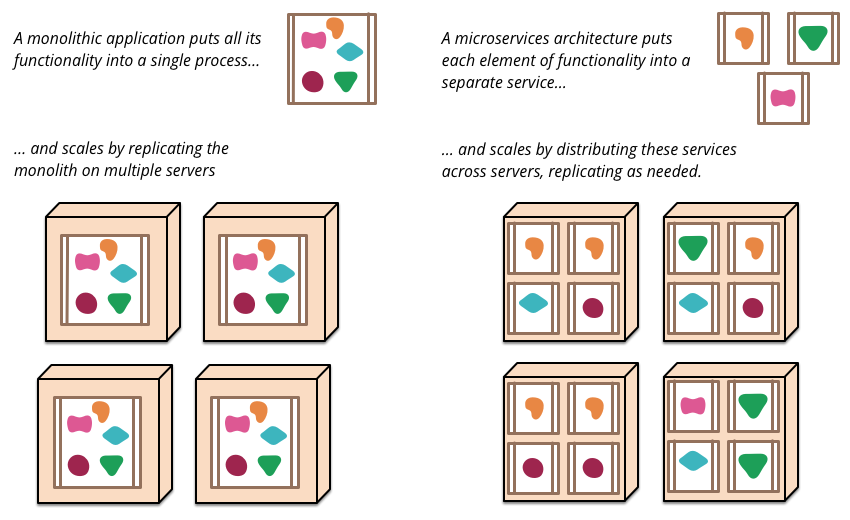
\includegraphics{assets/figures/microservices.png}
   }
   \caption[Monoliths and Microservices]{Monoliths and Microservices by \cite{martinmicro}}
   \label{fig:design:alternatives:auth:backend:scale}
\end{figure}

The final decision was to follow an architecture based on Microservices, even tho this decision had several oversights:

\begin{itemize}
   \item Development Team size: microservices are commonly adopted by big companies where each team of developers is responsible for a subset of microservices. This lowers the friction between teams when developing and deploying the solution and is seen as a big reason to move to a microservice architecture. For this solution, a single developer is responsible for everything;
   \item Time to Market: microservices need to interact with each other though the network. This added demand takes time to design and develop when compared to a monolith solution where communication is done via code;
   \item A solution shouldn't start with a microservice architecture: a solution should migrate to microservices when it becomes too complex and hard to maintain, \cite{ibmmicro}.
\end{itemize}

The decision made was based on the following assumptions, perceptions and findings:

\begin{itemize}
   \item There are well defined boundaries between the various business processes that the project needs to support;
   \item There is a perception that the solution will need to scale early on the road due to high volumes of \gls{IoT} data to process and store;
   \item There are a high number of completely independent External services to develop and deploy;
   \item There are different types of costumers with diverse requirements regarding the deployment and development of the solution;
   \item Each costumer is interested in their specific business case or cases and therefore requires different combinations of External Services.
\end{itemize}

\gls{SOA} was discarded since: ``Although the concept of a share-as-much-as-possible architecture solves issues associated with the duplication of business functionality, it also tends to lead to tightly coupled components and increases the overall risk associated with change''. (\cite{richards2015microservices}). Microservices are more easily extended when/if needed compared with \gls{SOA} since the focus is on loose coupling services and not highly reusable services.

Despite this, the solution adopted some architecture decisions that are usually associated with \gls{SOA}, as an example a canonical data model (Section~\ref{subsec:design:domain:shared_model}) was created to ease the communication between services. This is something common in projects that follow \gls{SOA} according to \cite{cerny2017disambiguation}.

\subsection{Frontend Segregation}
\label{subsec:design:alternatives:frontend}

This section tackles the need for segregating the frontend into various independent frontends - Microfrontends, \cite{microfrontends} - or to develop a single Frontend to answer the identified requirements.

The non-functional requirements discussed in Section~\ref{sec:requirements:non_functional} enhance the need to develop a product that can be fully extensible and yet close for modifications, following the idea behind the \gls{OCP} (introduced by \cite{martin2003agile}). This need arises so that costumer entities can easily create new \gls{IoT} services without the need to alter any close source code that is produced internally.

The Microfrontends Architecture when applied to this project has the same oversights, assumptions and perceptions that lead to the decision taken in the \nameref{subsec:design:alternatives:backend} Section. As such, the decision was to drop the design and development of a single frontend in favor of a Microfrontends Architecture.

Ultimately this decision, coupled with the Backend Segregation decision made, enforces a business model that follows \gls{OCP} and simplifies the adoption of this solution by third parties.

\subsection{User Authentication/Authorization}
\label{subsec:design:alternatives:auth}

User Authentication/Authorization is an important aspect of the solution. During the requirements elicitation, mentioned in Section~\ref{subsec:requirements:functional:roles}, it was clear that several different levels of permissions had to be given to Tenants. These levels of permissions also had to be managed by someone. As such, users had to be authenticated in the system and all accesses had to be authorized.

Four approaches were considered:

\begin{itemize}
   \item \nameref{subsubsec:design:alternatives:auth:internalauth};
   \item \nameref{subsubsec:design:alternatives:auth:externalauth};
   \item \nameref{subsubsec:design:alternatives:auth:externalauthinternalpermission};
   \item \nameref{subsubsec:design:alternatives:auth:externalauthinternaloauth}.
\end{itemize}

The fourth option was the approach taken.

\subsubsection{Internal Authentication Server}
\label{subsubsec:design:alternatives:auth:internalauth}

By creating an Internal Authentication Server we could have a normal, private and controlled user authentication/authorization flow in the environment. Both user credentials and permissions would be managed internally.

The following diagram, Figure~\ref{fig:design:alternatives:auth:internalauth:diagram},presents the normal environment flow for this alternative.

\begin{figure}[H]
   \centering
   \resizebox{\columnwidth}{!}
   {
      \input{assets/diagrams/design/alternatives/auth/alternative1.latex}
   }
   \caption[User Authentication/Authorization - Internal Authentication Server Alternative - Sequence Diagram]{User Authentication/Authorization - Internal Authentication Server Alternative - Sequence Diagram}
   \label{fig:design:alternatives:auth:internalauth:diagram}
\end{figure}

This alternative introduces the need to internally secure user credentials and other sensitive information from data breaches. It would also require each user to register in sensae with a new account credentials. For this reasons this alternative was discarded.

\subsubsection{External Authentication Server}
\label{subsubsec:design:alternatives:auth:externalauth}

By using an External Authentication Server there would be no need to store user credentials or permissions. This services are commonly identified as \gls{CIAM} solutions. According to \cite{ciam} these solutions include features such as ``self-service for registration, password and consent management, profile generation and management, authentication and authorization into applications, identity repositories, reporting and analytics, APIs and SDKs for mobile applications, and social identity registration and login''.

The following diagram, Figure~\ref{fig:design:alternatives:auth:externalauth:diagram}, presents the normal environment flow for this alternative.

\begin{figure}[H]
   \centering
   \resizebox{\columnwidth}{!}
   {
      \input{assets/diagrams/design/alternatives/auth/alternative2.latex}
   }
   \caption[User Authentication/Authorization - External Authorization Server Alternative - Sequence Diagram]{User Authentication/Authorization - External Authorization Server Alternative - Sequence Diagram}
   \label{fig:design:alternatives:auth:externalauth:diagram}
\end{figure}

This approach would create a strong dependency to the \gls{CIAM} solution used since all user credentials and authorization level would have to be managed by the \gls{CIAM} solution.
Some of this services are: (i) \citetitle{auth0id}, (ii) \citetitle{googleid}, (iii) \citetitle{oktaid}, (iv) \citetitle{amazonid} and (v) \citetitle{azureid}.

The platform Auth0 was tested and is capable of answering all of this project's requirements.

As stated before, the dependency created would force the environment to always be coupled to the chosen \gls{CIAM} solution. For this reason this alternative was discarded.

\subsubsection{External Authentication Server with Internal Authorization Server}
\label{subsubsec:design:alternatives:auth:externalauthinternalpermission}

By using an External Authentication Server there would be no need to store user credentials, the user authorization aspects would then be managed internally via and \textit{Authorization Server}.

The following diagram, Figure~\ref{fig:design:alternatives:auth:externalauthinternalpermission:diagram}, presents the normal environment flow for this alternative.

\begin{figure}[H]
   \centering
   \resizebox{\columnwidth}{!}
   {
      \input{assets/diagrams/design/alternatives/auth/alternative3.latex}
   }
   \caption[User Authentication/Authorization - External Authentication Server with Internal Authorization Server Alternative - Sequence Diagram]{User Authentication/Authorization - External Authentication Server with Internal Authorization Server Alternative - Sequence Diagram}
   \label{fig:design:alternatives:auth:externalauthinternalpermission:diagram}
\end{figure}

This approach would create a dependency to the \gls{CIAM} solution used and presented in the second alternative.

This dependency is less severe compared with the second alternative since all authorization aspects would be managed internally.
This approach would require any backend to query the \textit{Authorization Server} for user permissions so that it could verify if the user was authorized to preform the requested action or not. This would therefore linger down the performance of the system since each action would have to be verified in a single container: the \textit{Authorization Server}.

\subsubsection{External Authentication Server with Internal Oauth2 Server}
\label{subsubsec:design:alternatives:auth:externalauthinternaloauth}

By using an external Authorization Server there would be no need to store user credentials. An internal Oauth2 Server would remove the direct dependency to the \textit{Permissions Server} presented in the third alternative.

This alternative is introduced in Figure~\ref{fig:design:architecture:container:process:diagram:authentication} and Figure~\ref{fig:design:architecture:container:process:diagram:authorization} where the Internal Oauth2 Server is the Identity Management Backend.

This approach would create a dependency to the \gls{CIAM} solution used and presented in the second alternative. This dependency is less severe compared with the second alternative since all user permissions would be managed internally.
This approach would require the system to create and refresh \textit{access tokens} based on the \textit{id token} received by the external \gls{CIAM} solution. Contrary to the third alternative it would not create excessive pressure in a specific container.

This approach also allows the system to easily integrate with more than one \gls{CIAM} solution while managing user permissions in a single place. The \gls{CIAM} solutions that \textbf{Sensae Console} is integrated with are:

\begin{itemize}
   \item Google Identity Platform: for common individuals that want to use the system, since almost everyone has a google account;
   \item Azure Active Directory: for companies and organizations since most use Office 365 services internally.
\end{itemize}

Due to the reasons presented above, this was the adopted approach.

\subsection{Data Flow Pipeline}
\label{subsec:design:alternatives:flow}

This section debates how the various Data Flow Containers should communicate with each other.

Synchronous communication, such as HTTP requests, was promptly discarded since there is no need for each Container to acknowledge the outcome of the Data Unit that it sent and this type of communication would linger the performance of the Data Flow Scope by creating chained requests, an anti pattern when using a Microservice Architecture [\cite{microsoftmicroanti}].

According to \cite{microsoftasync}, there are two kinds of asynchronous messaging communication: single receiver message-based communication, and multiple receivers message-based communication. It is common to use both of this types in the same solution depending on the requirements. This type of communication is usually composed by the following participants:

\begin{itemize}
   \item Broker: responsible for establishing a communication channel between Receivers and Publishers;
   \item Publishers: responsible for sending messages;
   \item Receivers: responsible for consuming messages.
\end{itemize}

Looking at the Figure~\ref{fig:design:architecture:container:process:diagram:flow} it appears that a simple \textit{single receiver message-based communication} would be sufficient but this approach isn't as flexible as other options. By following a \textit{multiple receivers message-based communication}, additional receivers can be added in the future without the need to modify the sender service. As an example, the Data Store container can be modified to consume any type of Data Unit without changing the containers that produce them.

The final issue to discuss is whether Receivers should pull messages from the Broker (via pulling) or the Broker should push messages to Receivers. This topic is discussed in \citetitle{pubsubpushpull}, mentioned as Push vs Pull. Pushing messages to Receivers can overwhelm a receiver when its rate of consumption falls below the rate of production. The Pull approach offers Receivers the option to consume messages at the rate that they are capable of but can be wasteful in systems where messages are not abundant [\cite{pubsubpushpullrab}]. The operations preformed in each Data Flow container are meant to be fast and simple, and as such overwhelming a receiver was not taken into consideration. The Push approach was preferred since it theoretically enables faster reactions to new message compared to the Push approach.

As such, it was decided that the Data Flow Pipeline would work based on the publish/subscribe pattern on top of asynchronous messaging communication. Messages would be published to a broker and then routed to consumers.

\subsection{Internal Communication}
\label{subsec:design:alternatives:internal}

This section tackles how the Data Flow Scope should be kept up to date on the configurations made in the Configuration Scope. Five alternatives have been discussed:

\begin{enumerate}
   \item Data Flow Containers directly access the Database related to their Context;
   \item Data Flow Containers request information to their context's Configuration Scope Container via synchronous calls;
   \item Data Flow Containers are feed updates to their context configurations via asynchronous calls and store this information;
   \item A shared, in memory, database is kept, Configuration Scope writes to it and Data Flow Scope queries information from it;
   \item An append-only log is used to store configuration logs, the Configuration Scope writes to it and the Data Flow Scope can always read from it.
\end{enumerate}

The third option was the approach taken.

\subsubsection{First Option}
\label{subsubsec:design:alternatives:internal:first}

This option ensures that the Data Flow Containers are kept updated by giving them direct access to the source of truth, the database. The logical view diagram in Figure~\ref{fig:design:alternatives:internal:first:diagram} describes how this option functions.

\begin{figure}[H]
   \centering
   \resizebox{\columnwidth}{!}
   {
      \input{assets/diagrams/design/alternatives/internal/alternative1.latex}
   }
   \caption[Internal Communication - First Option - Logical View Diagram]{Internal Communication - First Option - Logical View Diagram}
   \label{fig:design:alternatives:internal:first:diagram}
\end{figure}

This approach ensures that the Message Broker is only used to transport Data Units, Alerts and Commands, alleviating it from an heavy responsibility.
That responsibility is assigned to the \textit{X Context Flow} Container and the \textit{X Context Database} Container.
This approach has several drawbacks such as:

\begin{itemize}
   \item The \textit{X Context Flow} Container has full access to superfluous configuration details related to that context configuration;
   \item The same database access has to be developed and maintained in two separated containers;
   \item All database accesses are blocking calls by nature that would slow down the process;
   \item Data Flow containers can't reliably cache information collected since there is no way to know when the corresponding information was updated. Meaning that every time a new message arrives the database has to be queried.
\end{itemize}

Due to this drawbacks this option was eventually dropped.

\subsubsection{Second Option}
\label{subsubsec:design:alternatives:internal:second}

This option ensures that the Data Flow Containers are kept updated querying information from a \gls{REST} \gls{API} provided by the Configuration Containers. The logical view diagram in Figure~\ref{fig:design:alternatives:internal:second:diagram} describes how this option functions.

\begin{figure}[H]
   \centering
   \resizebox{\columnwidth}{!}
   {
      \input{assets/diagrams/design/alternatives/internal/alternative2.latex}
   }
   \caption[Internal Communication - Second Option - Logical View Diagram]{Internal Communication - Second Option - Logical View Diagram}
   \label{fig:design:alternatives:internal:second:diagram}
\end{figure}

This approach doesn't suffer from all drawbacks stated for the first option but still requires a blocking call to the \textit{X Context Backend} Container every time a new message arrives to the \textit{X Context Flow} Container.

It's an improvement of the first option but still has some serious drawbacks and therefore it was also abandoned.

\subsubsection{Third Option}
\label{subsubsec:design:alternatives:internal:third}

This option ensures that the Data Flow Containers are kept updated by allowing them to subscribe to changes made in their context's configuration. The logical view diagram in Figure~\ref{fig:design:alternatives:internal:third:diagram} describes how this option functions.

\begin{figure}[H]
   \centering
   \resizebox{\columnwidth}{!}
   {
      \input{assets/diagrams/design/alternatives/internal/alternative3.latex}
   }
   \caption[Internal Communication - Third Option - Logical View Diagram]{Internal Communication - Third Option - Logical View Diagram}
   \label{fig:design:alternatives:internal:third:diagram}
\end{figure}

The major improvement of this approach when compared with the options above is that, since \textit{X Context Flow} Container subscribes to configuration updates, it can reliably keep a cache with just the needed information (and not the entire context configuration). This works since \textit{X Context Flow} Containers can discard updates related to information that they currently don't use. Once the container needs that information, it can send an event requesting what it needs and that information arrives later as a normal update to the configuration.
All \textit{X Context Flow} external interactions also rely on asynchronous communication, ensuring a more robust performance.

The main drawback to this option is that the \textit{Message Broker} becomes responsible for yet another communication topic inside the environment.

Despite this drawback this is the option currently in use. The following options purpose alternatives to tackle this drawbacks.

\subsubsection{Fourth Option}
\label{subsubsec:design:alternatives:internal:fourth}

This option ensures that the Data Flow Containers are kept updated by allowing them to query information from an \textit{Internal State Database}. This approach differs from the first option since the \textit{Internal State Database} is supposed to be a fast in memory database with only the needed information for Data Flow Containers to process Data Units, Alerts and Commands. The logical view diagram in Figure~\ref{fig:design:alternatives:internal:fourth:diagram} describes how this option functions.

\begin{figure}[H]
   \centering
   \resizebox{\columnwidth}{!}
   {
      \input{assets/diagrams/design/alternatives/internal/alternative4.latex}
   }
   \caption[Internal Communication - Fourth Option - Logical View Diagram]{Internal Communication - Fourth Option - Logical View Diagram}
   \label{fig:design:alternatives:internal:fourth:diagram}
\end{figure}

This approach would remove the responsibly from the \textit{Message Broker} to maintaining the internal state updated in the Data Flow Scope.
The \textit{Internal State Database} would in turn store information that \textit{X Content Flow} could query.

The main drawbacks of this approach are the same stated in the second option, even tho they can be mitigated by leveraging technologies that tackle distributed caching problems.

\subsubsection{Fifth Option}
\label{subsubsec:design:alternatives:internal:fifth}

This option ensures that the Data Flow Containers are kept updated by allowing them to subscribe to changes made in their context's configuration. This option diverges from the third option since the event store would persist all updates to contexts configurations. The logical view diagram in Figure~\ref{fig:design:alternatives:internal:fifth:diagram} describes how this option functions.

\begin{figure}[H]
   \centering
   \resizebox{\columnwidth}{!}
   {
      \input{assets/diagrams/design/alternatives/internal/alternative5.latex}
   }
   \caption[Internal Communication - Fifth Option - Logical View Diagram]{Internal Communication - Fifth Option - Logical View Diagram}
   \label{fig:design:alternatives:internal:fifth:diagram}
\end{figure}

The \textit{X Context Flow} Container would use event sourcing to reach the current state of its context configuration on start up and then cache this state internally. New events would then be sent automatically via subscription to keep the state up-to-date.

The main drawback of this approach is that the container can't keep just the needed portion of configurations without recreating the entire state though event sourcing.


\section{Domain}
\label{sec:design:domain}

This solution's domain model will be discussed here. The idea behind this section is to introduce core business concepts to the reader and explain how they map to the contexts refereed before. To represent this ideas the \gls{UML} notation is used.

This section is split into four pieces: (i) concepts, (ii) shared model, (iii) sensae console bounded contexts and (iv) external services bounded contexts.

\subsection{Taxonomy}
\label{subsec:design:domain:taxonomy}

In order for the reader to better understand how the system operates, some concepts need to be better classified and explained:

\begin{itemize}
   \item \textbf{Device}: A device is a "Thing" that can collect data and submit it to \textbf{Sensae Console} via an external system though \textbf{Uplink}s (commonly refereed as a sensor). A device can also receive \textbf{Downlink}s and act base on what was received (commonly refereed as an actuator);
   \item \textbf{Controller}: A controller is a \textbf{Device} that controls and aggregates data from various sub \textbf{Device}s;
   \item \textbf{Records/Metadata}: Records, or Metadata are labels associated to a \textbf{Device} that help an organization to classify and add some context to the owned \textbf{Device}s;
   \item \textbf{Downlink}: A downlink is a term commonly used in radio communications to denote the transmission from the network to the end user. In this case the network is the \textbf{Sensae Console} and the end user is a \textbf{Device};
   \item \textbf{Uplink}: An uplink is the opposite of a \textbf{Downlink}, it's the transmission from a \textbf{Device} to the \textbf{Sensae Console};
   \item \textbf{Data Unit}: A data unit represents the collected measures that are atomically submitted via an \textbf{Uplink} to the \textbf{Sensae Console}. This data should be, at least, enriched with an unique identifier of the \textbf{Uplink} and \textbf{Device} that sent it. The data unit can contain measures captured by various devices, in that case the device is identified as a Controller;
   \item \textbf{Device Command}: A device command is an abstraction on top of a \textbf{Downlink} intended to instruct a \textbf{Device} to execute a specific action. This devices are commonly identified as actuators. As an example, one could send a command to open or close a valve that is incorporated into a \textbf{Device};
   \item \textbf{Decoder}: A decoder is a function that translates a \textbf{Data Unit} into something that \textbf{Sensae Console} understands;
   \item \textbf{Domain}: A domain represents a department in a organization. An organization is composed of several domains structured in a tree like format;
   \item \textbf{Tenant}: A tenant is a user that belongs to one or more \textbf{Domain}s and represents any of the roles discussed in Section~\ref{sec:requirements:functional};
   \item \textbf{Alert}: A report about a detected condition based on the gather \textbf{Data Unit};
   \item \textbf{Topic}: A Topic is a subcategory of the type of contents that are traded between the various containers in the system.
\end{itemize}

Currently the \textbf{Topic}s that flow in the system are:

\begin{itemize}
   \item \textbf{Data}: This topic references the \textbf{Data Unit} concept and is intended to be consumed by the \textbf{External Services Scope};
   \item \textbf{Command}: This topic references the \textbf{Device Command} concept and is intended to be used mainly by the \textbf{External Services Scope};
   \item \textbf{Alert}: This topic references the \textbf{Alert} concept and is intended to be consumed mainly by the \textbf{External Services Scope};
   \item \textbf{Internal}: This topic references the internal state maintained in the \textbf{Configuration Scope} and \textbf{Data Flow Scope}.
\end{itemize}

This concepts are referenced across the document.

\subsection{Shared Model}
\label{subsec:design:domain:shared_model}

The shared model is comprised of concepts that transverse the entire \textbf{Sensae Console} business model, and by extension any \textbf{External Service}. Therefore, it is built as a library, \textit{iot-core}, that can be used by entities that rely on the exchange of information with/inside \textbf{Sensae Console}. It can be seen as a domain that focus on defining the protocol of exchange of information between the various entities of the system.

The intent behind this Shared Model is to alleviate one of the issues related to distributed systems - heterogeneity in data formats (\cite{nadiminti2006distributed}) - and to provide a simple \gls{SDK} for third-parties to develop new external services that interact with \textbf{Sensae Console}. It can be seen as an explicit schema. According to \cite{explicitsharedmodel}, ``any implementation of event-based communication between a producer and consumer that lacks an explicit predefined schema will inevitably end up relying on an implicit schema. Implicit data contracts are brittle and susceptible to uncontrolled change, which can cause much undue hardship to downstream consumers.''

According to \cite{integration}, ``while we have historically drawn up our project plans and costs around the boxes — the digital products we are introducing — the lines are the hidden and often primary driver of organizational tech debt. They are the reason that things just take longer now than they used to.'' The \textit{'lines'} in this solution are a first class citizen and, instead of just linking the system together, they act as the pillars that shape the entire ecosystem.

It is comprised of three big components: (i) data model, (ii) message envelop model, and (iii) routing model.

\subsubsection{Data Model}
\label{subsubsec:design:domain:shared_model:data}

The data model represents the \textbf{Data Unit} that \textbf{Sensae Console} is currently capable of understanding. The following diagram, Figure~\ref{fig:design:domain:shared_model:data:diagram}, is a high level specification.

\begin{figure}[H]
   \centering
  \resizebox{\columnwidth}{!}
  {
     \input{assets/diagrams/design/domain/shared-model.latex}
  }
  \caption[Shared Model]{Shared Model}
  \label{fig:design:domain:shared_model:data:diagram}
\end{figure}

As a brief description:

\begin{itemize}
   \item \textbf{Data Unit} is the entry point to the shared model;
   \item The \textit{reportedAt} attribute represents an absolute timestamp of when the \textbf{Data Unit} was captured, in milliseconds;
   \item The \textit{Device} concept represents the \textbf{Device} that sent the \textit{Data Unit};
   \item The \textit{Record} concept represents an entry of \textbf{Records/Metadata};
   \item The \textit{Domain} concept references the \textbf{Domain} that owns the \textit{Device};
   \item The \textit{SubDeviceMeasures} referes to the collected measures. When the device is a Controller there's a need to map each sub device's measures with it and not with the Controller that sent the uplink. The \textit{reference} attribute indicates what sub device collected the measure, the reference \textit{zero} referes to the device that sent the uplink;
   \item The \textit{SubDeviceCommands} referes to the available commands to control the device. When the device is a Controller there's a need to map each sub device commands with it and not with the Controller that sent the uplink. The \textit{reference} attribute indicates the sub device that is controlled by the commands mentioned, the reference \textit{zero} referes to the device that sent the uplink;
   \item The \textit{Measures} concept contains various common data types related to \gls{IoT}.
\end{itemize}

As explained, \textit{Measures} contains various data types. Currently the supported types are presented in the Table~\ref{tab:design:domain:shared_model:data:data_types}. The team involved in this project decided what data types were needed to support based on the requested \gls{PoC}s and the purchased sensors. In the future more data types are expected to be included in the model.

\begin{landscape}
   \begin{longtable}{cllll}
   \caption{Measure Data Types}
   \label{tab:design:domain:shared_model:data:data_types}\\
   \cline{1-4}
   \multicolumn{2}{l}{\textbf{Data Type}}                                     & \multirow{2}{*}{\textbf{Description}}                  & \multirow{2}{*}{\textbf{Unit}} &  \\
   \textit{Property}                     & \textit{Sub Property}              &                                                        &                                &  \\ \cline{1-4}
   \endfirsthead
   %
   \multicolumn{5}{c}%
   {{\bfseries Table \thetable\ continued from previous page}} \\
   \cline{1-4}
   \multicolumn{2}{l}{\textbf{Data Type}}                                     & \multirow{2}{*}{\textbf{Description}}                  & \multirow{2}{*}{\textbf{Unit}} &  \\
   \textit{Property}                     & \textit{Sub Property}              &                                                        &                                &  \\ \cline{1-4}
   \endhead
   %
   \\
   \cline{1-4}
   \\
   \endfoot
   %
   \endlastfoot
   %
   \\[-0.85em]
   \multicolumn{2}{l}{\textbf{Trigger}}                                       & \multicolumn{2}{l}{Type related to something with an on / off or open / close state}    &  \\
   \textit{trigger}                      & \textit{value}                     & Value can be true or false                                    & boolean                        &  \\ [0.4em] \cline{1-4}
   \\[-0.85em]
   \multicolumn{2}{l}{\textbf{Motion}}                                        & \multicolumn{2}{l}{Status related to the motion of a device}                            &  \\
   \textit{motion}                       & \textit{value}                     & Value can be "ACTIVE", "INACTIVE" or "UNKNOWN"         & n.a.                           &  \\ [0.4em] \cline{1-4}
   \\[-0.85em]
   \multicolumn{2}{l}{\textbf{Velocity}}                                      & \multicolumn{2}{l}{How fast a device is moving}                                         &  \\
   \textit{velocity}                     & \textit{kilometerPerHour}          & Value measured in                                      & km/h                           &  \\ [0.4em] \cline{1-4}
   \\[-0.85em]
   \multicolumn{2}{l}{\textbf{Temperature}}                                   & \multicolumn{2}{l}{Temperature measured by a device}                                    &  \\
   \textit{temperature}                  & \textit{celsius}                   & Value measured in                                      & celsius                        &  \\ [0.4em] \cline{1-4}
   \\[-0.85em]
   \multicolumn{2}{l}{\textbf{AQI}}                                           & \multicolumn{2}{l}{Air Quality Index according to the U.S. AQI}                         &  \\
   \textit{aqi}                          & \textit{value}                     & Value measured in                                      & AQI                            &  \\ [0.4em] \cline{1-4}
   \\[-0.85em]
   \multicolumn{2}{l}{\textbf{Air Pressure}}                                  & \multicolumn{2}{l}{Pressure within the atmosphere of Earth}                             &  \\
   \textit{airPressure}                  & \textit{hectoPascal}               & Value measured in                                      & hPa                            &  \\ [0.4em] \cline{1-4}
   \\[-0.85em]
   \multicolumn{2}{l}{\textbf{Distance}}                                      & \multicolumn{2}{l}{Distance measured from the device to a surface}                      &  \\
   \multirow{3}{*}{\textit{distance}}    & \textit{millimeters}               & Value measured in                                      & mm                             &  \\
                                         & \textit{maxMillimeters}            & Maximum distance the sensor can be to a given surface  & mm                             &  \\
                                         & \textit{minMillimeters}            & Minimum distance the sensor can be to a given surface  & mm                             &  \\ [0.4em] \cline{1-4}
   \\[-0.85em]
   \multicolumn{2}{l}{\textbf{Soil Moisture}}                                 & \multicolumn{2}{l}{Amount of water, including water vapor, in an unsaturated soil}      &  \\
   \textit{soilMoisture}                  & \textit{relativePercentage}        & Value measured in                                      & \%                             &  \\ [0.4em] \cline{1-4}
   \\[-0.85em]
   \multicolumn{2}{l}{\textbf{Water Pressure}}                                & \multicolumn{2}{l}{Water Pressure measured in pipes by a device}                        &  \\
   \textit{waterPressure}                & \textit{bar}                       & Value measured in                                      & bar                            &  \\ [0.4em] \cline{1-4}
   %\pagebreak
   \\[-0.85em]
   \multicolumn{2}{l}{\textbf{Illuminance}}                                   & \multicolumn{2}{l}{Illuminance level - luminous flux per unit area}                     &  \\
   \textit{illuminance}                  & \textit{lux}                       & Value measured in                                      & lux                            &  \\ [0.4em] \cline{1-4}
   \\[-0.85em]
   \multicolumn{2}{l}{\textbf{CO2}}                                           & \multicolumn{2}{l}{Atmospheric Carbon Dioxide concentration}                            &  \\
   \textit{co2}                          & \textit{ppm}                       & Value measured in                                      & ppm                            &  \\ [0.4em] \cline{1-4}
   \\[-0.85em]
   \multicolumn{2}{l}{\textbf{CO}}                                            & \multicolumn{2}{l}{Atmospheric Carbon Oxide concentration}                              &  \\
   \textit{co}                           & \textit{ppm}                       & Value measured in                                      & ppm                            &  \\ [0.4em] \cline{1-4}
   \\[-0.85em]
   \multicolumn{2}{l}{\textbf{VOC}}                                           & \multicolumn{2}{l}{Volatile Organic Compounds concentration measured by a device}       &  \\
   \textit{voc}                          & \textit{ppm}                       & Value measured in                                      & ppm                            &  \\ [0.4em] \cline{1-4}
   \\[-0.85em]
   \multicolumn{2}{l}{\textbf{NH3}}                                           & \multicolumn{2}{l}{Atmospheric Ammonia concentration}                                   &  \\
   \textit{nh3}                          & \textit{ppm}                       & Value measured in                                      & ppm                            &  \\ [0.4em] \cline{1-4}
   \\[-0.85em]
   \multicolumn{2}{l}{\textbf{O3}}                                            & \multicolumn{2}{l}{Atmospheric Ozone concentration measured by a device}                &  \\
   \textit{o3}                           & \textit{ppm}                       & Value measured in                                      & ppm                            &  \\ [0.4em] \cline{1-4}
   \\[-0.85em]
   \multicolumn{2}{l}{\textbf{NO2}}                                           & \multicolumn{2}{l}{Atmospheric Nitrogen dioxide concentration}                          &  \\
   \textit{no2}                          & \textit{ppm}                       & Value measured in                                      & ppm                            &  \\ [0.4em] \cline{1-4}
   \\[-0.85em]
   \multicolumn{2}{l}{\textbf{PM2.5}}                                         & \multicolumn{2}{l}{Particulate Matter in the air (size up to 2.5 micrometers)}          &  \\
   \textit{pm2\_5}                       & \textit{microGramsPerCubicMeter}   & Value measured in                                      & $\mu$g/m3                      &  \\ [0.4em] \cline{1-4}
   \\[-0.85em]
   \multicolumn{2}{l}{\textbf{PM10}}                                          & \multicolumn{2}{l}{Particulate Matter in the air (size up to 10 micrometers)}           &  \\
   \textit{pm10}                         & \textit{microGramsPerCubicMeter}   & Value measured in                                      & $\mu$g/m3                      &  \\ [0.4em] \cline{1-4}
   \\[-0.85em]
   \multicolumn{2}{l}{\textbf{pH}}                                            & \multicolumn{2}{l}{Scale used to specify how acidic or basic a water-based solution is} &  \\
   \textit{ph}                           & \textit{value}                     & Value between 0 and 14 measured in                     & pH                             &  \\ [0.4em] \cline{1-4}
   \\[-0.85em]
   \multicolumn{2}{l}{\textbf{Occupation}}                                    & Occupation percentage measured inside a vessel         &                                &  \\
   \textit{occupation}                   & \textit{percentage}                & Value measured in                                      & \%                             &  \\ [0.4em] \cline{1-4}
   \\[-0.85em]
   \multicolumn{2}{l}{\textbf{Soil Conductivity}}                             & \multicolumn{2}{l}{Substances ability to conduct an electrical current in the soil}     &  \\
   \textit{soilConductivity}             & \textit{microSiemensPerCentimeter} & Value measured in                                      & $\mu$S/cm                      &  \\ [0.4em] \cline{1-4}
   \\[-0.85em]
   \multicolumn{2}{l}{\textbf{Air Humidity}}                                  & \multicolumn{2}{l}{Concentration of water vapour present in the air}                    &  \\
   \multirow{2}{*}{\textit{airHumidity}} & \textit{gramsPerCubicMeter}        & Value measured in                                      & g/m3                           &  \\
                                         & \textit{relativePercentage}        & Value measured in                                      & \%                             &  \\ [0.4em] \cline{1-4}
   \\[-0.85em]
   \multicolumn{2}{l}{\textbf{GPS}}                                           & \multicolumn{2}{l}{Point reference in the Geographic Coordinate System}                 &  \\
   \multirow{3}{*}{\textit{gps}}         & \textit{latitude}                  & Value between -90 and 90 measured in                   & degrees                        &  \\
                                         & \textit{longitude}                 & Value between -180 and 180 measured in                 & degrees                        &  \\
                                         & \textit{altitude}                  & Value determined according to the mean sea level       & meters                         &  \\ [0.4em] \cline{1-4}
   \\[-0.85em]
   \multicolumn{2}{l}{\textbf{Battery}}                                       & \multicolumn{2}{l}{Battery of the device}                                               &  \\
   \multirow{4}{*}{\textit{battery}}     & \textit{volts}                     & Value measured in                                      & volts                          &  \\
                                         & \textit{percentage}                & Value measured in                                      & \%                             &  \\
                                         & \textit{maxVolts}                  & Minimum volts the battery needs for the device to work & volts                          &  \\
                                         & \textit{minVolts}                  & Maximum volts the battery can hold                     & volts                          &  \\ [0.4em] \cline{1-4}
   \end{longtable}
\end{landscape}

The full json-like model schema can be found in Appendix~\ref{AppendixA}.

\subsubsection{Message Envelop Model}
\label{subsubsec:design:domain:shared_model:message}

The message envelop model refers to how, coupled with the routing model in Section~\ref{subsubsec:design:domain:shared_model:routing}, information can reliably transverse the system.

The diagram present in Figure~\ref{fig:design:domain:shared_model:messsage:diagram} details this model.

\begin{figure}[H]
   \centering
  \resizebox{\columnwidth}{!}
  {
     \input{assets/diagrams/design/domain/message-envelop-model.latex}
  }
  \caption[Message Envelop Model]{Message Envelop Model}
  \label{fig:design:domain:shared_model:messsage:diagram}
\end{figure}

As a brief description:

\begin{itemize}
   \item A \textit{MessageSupplied} is created in a issuer system and supplied to start the flow of information in the system;
   \item A \textit{MessageConsumed} is consumed by a consumer system and can then be transformed into a \textit{MessageSupplied} to be supplied;
   \item \textit{Information} represents the content of the message;
   \item \textit{RoutingKeys} represents the model referenced in Section~\ref{subsubsec:design:domain:shared_model:routing};
\end{itemize}

This concept is mainly used to ensure that information flowing in the system is not reprocessed, by verifying the unique id - \textit{oid}, and is eliminated if it enters a routing loop by verifying that the \textit{hops} have not reached a maximum value.

\subsubsection{Routing Model}
\label{subsubsec:design:domain:shared_model:routing}

The routing model refers to how information can be routed through the system based on various parameters. The initial and current idea is based on the \textit{pub/sub} pattern, as discussed by \cite{urquhart2021flow}. Containers subscribe to information in a \textbf{Topic} with specific \textit{RoutingKey}s and publish information with \textit{RoutingKey}s.

The diagram present in Figure~\ref{fig:design:domain:shared_model:routing:diagram} details this model.

\begin{figure}[H]
   \centering
  \resizebox{\columnwidth}{!}
  {
     \input{assets/diagrams/design/domain/routing-model.latex}
  }
  \caption[Routing Model]{Routing Model}
  \label{fig:design:domain:shared_model:routing:diagram}
\end{figure}

As a brief description:

\begin{itemize}
   \item \textit{RoutingKeys} is the concept referenced in Figure~\ref{fig:design:domain:shared_model:messsage:diagram} and represents a collection of different \textit{RoutingKeyOption}s;
   \item There are currently 4 types of \textit{RoutingKeys}, one for each \textbf{Topic} (according to \nameref{subsec:design:domain:taxonomy});
   \item To ensure that the various containers in \textbf{Sensae Console} understand each other, a \textit{ProtocolVersionOptions} is provided. This concept follows the Semantic Versioning Specification 2.0 (\cite{semver}) an is assembled according to the version of \textit{iot-core} imported by the container;
   \item There are multiple \textit{RoutingKey} types not displayed in the diagram for brevity.
   \item The \textit{RoutingKeysBuilder} implements the \textit{Builder} pattern and its single responsibility is to validate and create \textit{RoutingKeys};
   \item A \textit{RoutingKeyOption} can have the value \textit{any}, if the \textit{RoutingKeysBuilderOptions} has the value \textit{CONSUMER}. This provides a 'relaxed' mode, for containers that consume/subscribe to messages and a 'strict' mode, where all \textit{RoutingKey} must be specified, for containers that supply/publish messages;
   \item \textit{NH3DataOptions} and \textit{ChannelOptions} are two examples of \textit{RoutingKey}, both used in the Data Topic.
\end{itemize}

In the Table~\ref{tab:design:domain:shared_model:routing} all currently used \textit{RoutingKey} are presented.

\begin{landscape}
   \begin{longtable}{cll}
   \caption{Routing Options}
   \label{tab:design:domain:shared_model:routing}\\
   \cline{1-2}
   \multicolumn{1}{l}{\textbf{Topic}}      & \multirow{2}{*}{\textbf{Description}}                                                                     &  \\
   \textit{Routing Key}                    &                                                                                                           &  \\ \cline{1-2}
   \endfirsthead
   %
   \multicolumn{3}{c}%
   {{\bfseries Table \thetable\ continued from previous page}} \\
   \cline{1-2}
   \multicolumn{1}{l}{\textbf{Topic}}      & \multirow{2}{*}{\textbf{Description}}                                                                     &  \\
   \textit{Routing Key}                    &                                                                                                           &  \\ \cline{1-2}
   \endhead
   %
   \cline{1-2}
   \endfoot
   %
   \endlastfoot
   %
   \multicolumn{1}{l}{\textbf{Common}}     & Routing Keys that belong to every Topic                                                                   &  \\
   \textit{Protocol Version Options}       & Version of the used \textit{iot-core} package                                                             &  \\
   \textit{Container Type Options}         & Type of the Container that published the message                                                          &  \\
   \textit{Ownership Options}              & Does the message contains the \textbf{Domain}s that own it\footnotemark[1]                                &  \\
   \textit{Topic Type Options}             & Topic used to publish the message                                                                         &  \\ \cline{1-2}
   \multicolumn{1}{l}{\textbf{Internal}}   & Routing Keys that belong to the Internal Topic                                                            &  \\
   \textit{Operation Type Options}         & Intent of the message, e.g. unknown context found                                                         &  \\
   \textit{Context Type Options}           & Type of content in the message, e.g. device information                                                   &  \\ \cline{1-2}
   \multicolumn{1}{l}{\textbf{Data}}       & Routing Keys that belong to the Data Topic                                                                &  \\
   \textit{Info Type Options}              & How data is shaped: (i) ENCODED, (ii) DECODED and (iii) PROCESSED                                         &  \\
   \textit{Device Type Options}            & Type of device, e.g. LGT-92 or EM300-TH                                                                   &  \\
   \textit{Channel Options}                & Name of channel where data flows, e.g. \textit{smartIrrigation} or \textit{default}                       &  \\
   \textit{Data Legitimacy Options}        & Is the data legitimate: (i) UNKNOWN, (ii) CORRECT, (iii) INCORRECT and (iv) UNDETERMINED      &  \\
   \textit{Records Options}                & Does the data contains \textbf{Records/Metadata}\footnotemark[1]                                          &  \\
   \textit{Air Humidity Data Options}      & Does the data contains information about Air Humidity\footnotemark[1]\footnotemark[2]                     &  \\
   \textit{Air Pressure Data Options}      & Does the data contains information about Air Pressure\footnotemark[1]\footnotemark[2]                     &  \\
   \textit{Air Quality Data Options}       & Does the data contains information about Air Quality\footnotemark[1]\footnotemark[2]                      &  \\
   \textit{Battery Data Options}           & Does the data contains information about the device Battery\footnotemark[1]\footnotemark[2]               &  \\
   \textit{CO2 Data Options}               & Does the data contains information about CO2 levels\footnotemark[1]\footnotemark[2]                       &  \\
   \textit{CO Data Options}                & Does the data contains information about CO levels\footnotemark[1]\footnotemark[2]                        &  \\
   \textit{Distance Data Options}          & Does the data contains information about distances to a surface\footnotemark[1]\footnotemark[2]           &  \\
   \textit{GPS Data Options}               & Does the data contains information about the device GPS coordinates\footnotemark[1]\footnotemark[2]       &  \\
   \textit{Illuminance Data Options}       & Does the data contains information about illuminance in the environment\footnotemark[1]\footnotemark[2]   &  \\
   \textit{Motion Data Options}            & Does the data contains information about the device motion\footnotemark[1]\footnotemark[2]                &  \\
   \textit{NH3 Data Options}               & Does the data contains information about NH3 levels\footnotemark[1]\footnotemark[2]                       &  \\
   \textit{NO2 Data Options}               & Does the data contains information about NO2 levels\footnotemark[1]\footnotemark[2]                       &  \\
   \textit{O3 Data Options}                & Does the data contains information about O3 levels\footnotemark[1]\footnotemark[2]                        &  \\
   \textit{Occupation Data Options}        & Does the data contains information about occupation levels\footnotemark[1]\footnotemark[2]                &  \\
   \textit{pH Data Options}                & Does the data contains information about ph level\footnotemark[1]\footnotemark[2]                         &  \\
   \textit{PM2.5 Data Options}             & Does the data contains information about pm 2.5 concentration\footnotemark[1]\footnotemark[2]             &  \\
   \textit{PM10 Data Options}              & Does the data contains information about pm 10 concentration\footnotemark[1]\footnotemark[2]              &  \\
   \textit{Soil Conductivity Data Options} & Does the data contains information about the soil conductivity\footnotemark[1]\footnotemark[2]            &  \\
   \textit{Soil Moisture Data Options}     & Does the data contains information about the soil moisture\footnotemark[1]\footnotemark[2]                &  \\
   \textit{Temperature Data Options}       & Does the data contains information about the temperature\footnotemark[1]\footnotemark[2]                  &  \\
   \textit{Trigger Data Options}           & Does the data contains information about something that works as a switch\footnotemark[1]\footnotemark[2] &  \\
   \textit{Velocity Data Options}          & Does the data contains information about the device velocity\footnotemark[1]\footnotemark[2]              &  \\
   \textit{VOC Data Options}               & Does the data contains information about VOC concentration\footnotemark[1]\footnotemark[2]                &  \\
   \textit{Water Pressure Data Options}    & Does the data contains information about water pressure\footnotemark[1]\footnotemark[2]                   &  \\ \cline{1-2}
   \multicolumn{1}{l}{\textbf{Command}}    & Routing Keys that belong to the Command Topic                                                             &  \\
   \textit{Command Type Options}           & Type of command, e.g. Open Valve                                                                          &  \\ \cline{1-2}
   \multicolumn{1}{l}{\textbf{Alert}}      & Routing Keys that belong to the Alert Topic                                                               &  \\
   \textit{Alert Category Options}         & Category of the alert published, e.g. Fire Detention                                                      &  \\
   \textit{Alert Subcategory Options}      & Category of the alert published, e.g. Humidity With High Rate Of Change                                   &  \\
   \textit{Alert Severity Options}         & Severity of the alert published, from \textit{Information} level to \textit{Critical} level               &  \\ \cline{1-2}
   \end{longtable}
   \footnotetext[1]{has three possible values: (i) UNDETERMINED, (ii) WITH, (iii) WITHOUT}
   \footnotetext[2]{related to the explored Data Types}
\end{landscape}

The routing key \textit{OperationType} from the \textbf{Internal} topic can have the following values:

\begin{itemize}
   \item \textbf{Sync}: message contains the current state of the related \textit{ContextType}, used to populate a container's state;
   \item \textbf{Info}: message contains information about an entry of the related \textit{ContextType}, e.g. entry X in context Y was removed;
   \item \textbf{Unknown}: message contains entry of the related \textit{ContextType} that the container that published the message can't identify;
   \item \textbf{Init}: message to notify that a container has initiated and needs the current state of the related \textit{ContextType} to be ready;
   \item \textbf{Ping}: message to notify that an entry of the related \textit{ContextType} was used, e.g. entry X in context Y was just used.
\end{itemize}

The \textit{ContextType}, used to identity what piece of the state is referenced, can currently have the following values: (i) \textit{Data Processor}, (ii) \textit{Data Decoder}, (iii) \textit{Device Information}, (iv) \textit{Device Identity}, (v) \textit{Tenant Identity}, (vi) \textit{Addressee Configuration} and (vii) \textit{Rule Management}.

Routing keys help to strengthen the boundaries that a container is expected to have. As an example, a Service in the \textbf{External Services Scope} related to Waste Management would subscribe to the \textit{Data Topic} with the following \textit{Routing Keys}:

\begin{itemize}
   \item \textit{Info Type Options}: PROCESSED;
   \item \textit{Channel Options}: 'wasteManagement';
   \item \textit{Data Legitimacy Options}: CORRECT;
   \item \textit{GPS Data Options}: WITH;
   \item \textit{Occupation Data Options}: WITH;
   \item \textit{Records Options}: WITH;
   \item \textit{Ownership Options}: WITH;
\end{itemize}

And would, for example, subscribe to the \textit{Alert Topic} with the following \textit{Routing Keys}:

\begin{itemize}
   \item \textit{Alert Category Options}: 'wasteManagement';
   \item \textit{Alert SubCategory Options}: 'garbageFull';
   \item \textit{Ownership Options}: WITH;
\end{itemize}

As expected, the structure and semantics of the information subscribed to are known upfront with the help of the package \textit{iot-core}. The services developed and their pre-defined boundaries regarding data types consumed are detailed in Section~\ref{subsec:implementation:description:services}.

\subsection{Sensae Console Bounded Context}
\label{subsec:design:domain:bounded_contexts}

The \textbf{Bounded Context} concept, defined by \cite{evans2014domain}, refers to an unified model - with well-defined boundaries and internally consistent - that is, a single piece in a larger system composed by various bounded contexts.

The concept \textbf{Bounded Context} refereed in this section draws inspiration from the one coined by \cite{evans2014domain}, without the notion of Aggregates, Value Objects, Aggregate Root and other \gls{DDD} concepts. It is here to simply characterize the various models of the system that, when isolated, can be more clearly interpreted and understood by the reader.

For \textbf{Sensae Console}, each bounded context can be pictured as a core business process of the system, it is composed by the following:

\begin{itemize}
   \item Data Processor;
   \item Data Decoder;
   \item Device Management;
   \item Identity Management;
   \item Rule Management.
\end{itemize}

Each of this contexts will be briefly addressed in the following sections.

\subsubsection{Data Processor}
\label{subsubsec:design:domain:bounded_contexts:processor}

The \textbf{Data Processor} context refers to simple data mappers that translate inbound information to \textbf{Data Unit}s, discussed in Section~\ref{subsubsec:design:domain:shared_model:data}.

The received information must be \textit{decoded}, meaning that the inbound information simply has a different structure than \textbf{Data Unit}.

The diagram in Figure~\ref{fig:design:domain:bounded_contexts:processor:diagram} displays the noteworthy concepts in this context.

\begin{figure}[H]
   \centering
  \resizebox{\columnwidth}{!}
  {
     \input{assets/diagrams/design/domain/data-processor-model.latex}
  }
  \caption[Data Processor Context Model]{Data Processor Context Model}
  \label{fig:design:domain:bounded_contexts:processor:diagram}
\end{figure}

As a brief description:

\begin{itemize}
   \item \textbf{DataMapper}, the root entity in this context is identified by a \textbf{DeviceTypeId} and has various instructions to map properties from the inbound information to a \textbf{Data Unit} properties;
   \item \textbf{DeviceTypeId} identifies the type of device that can be processed by this data mapper. When a data unit's message is supplied to this context the data mapper that has the \textbf{DeviceTypeId} equal to the message's \textit{Device Type Options} routing key (mentioned in Table~\ref{tab:design:domain:shared_model:routing}) is used to process that data unit;
   \item \textbf{SubDeviceReference} represents a number that will be used later to reference a sub device when dealing with \textbf{Controller}s. For simple \textbf{Devices} the used and default value is \textit{0};
   \item \textbf{PropertyName} has much more properties that haven't been presented for brevity.
\end{itemize}

As an example, consider the inbound information represented as a JSON document with the structure in the example \ref{code:design:domain:bounded_contexts:processor:json}. To map the \textit{temperature} value to the \textbf{TEMPERATURE\_CELSIUS} property of a \textbf{Data Unit}, the \textbf{EncodedDataPropertyPath} would be \textit{decoded.data[0].temperature}.

\begin{lstlisting}[caption=Inbound Information Example, label={code:design:domain:bounded_contexts:processor:json}]
{
   "uuid": "de1a9d15-c018-4547-8453-87111cb4f81b",
   "id": "d81e6e69-1955-48a1-a1dd-4c812c15ebac",
   "time": 1657646955748,
   "decoded": {
      "data": [
         {
            "temperature": 18,
         }
      ]
   }
}
\end{lstlisting}

This process is simple since it expects the inbound information to be predisposed, but when working with \gls{IoT} Devices, to optimize the bandwidth used, it is common to send information encoded. The following section presents an alternative to this process.

\subsubsection{Data Decoder}
\label{subsubsec:design:domain:bounded_contexts:decoder}

The \textbf{Data Decoder} context refers to a more complex data mapper that translates inbound information to \textbf{Data Unit}s, discussed in Section~\ref{subsubsec:design:domain:shared_model:data}.
It was created to deal with the limitations mentioned in Section~\ref{subsubsec:design:domain:bounded_contexts:processor}.

The received information is usually \textit{encoded}, meaning that the inbound information is received as it was sent by the \textbf{Device}, commonly as a \textit{Base64} encoded string, that needs to be processed so that information can be extracted.

The diagram in Figure~\ref{fig:design:domain:bounded_contexts:decoder:diagram} displays the noteworthy concepts in this context.

\begin{figure}[H]
   \centering
  \resizebox{\columnwidth}{!}
  {
     \input{assets/diagrams/design/domain/data-decoder-model.latex}
  }
  \caption[Data Decoder Context Model]{Data Decoder Context Model}
  \label{fig:design:domain:bounded_contexts:decoder:diagram}
\end{figure}

As a brief description:

\begin{itemize}
   \item \textbf{DataDecoder}, the root entity in this context is identified by a \textbf{DeviceTypeId} and has a \textbf{Script};
   \item Currently, a \textbf{Script} can only be written in \textit{JavaScript} but in the future more languages like \textit{Python} or \textit{Groovy} can be added;
   \item The \textbf{ScriptContent} contains the code that will run for each inbound information that matches the \textbf{DeviceTypeId}.
\end{itemize}

This process requires some knowledge of the \textit{Javascript} language but it's much more flexible than the \textbf{Data Processor} operation.

\subsubsection{Device Management}
\label{subsubsec:design:domain:bounded_contexts:device}

The \textbf{Device Management} context refers to the inventory of all registered \textbf{Device}s in the \textbf{Sensae Console}.

The diagram in Figure~\ref{fig:design:domain:bounded_contexts:device:diagram} displays the noteworthy concepts in this context.

\begin{figure}[H]
   \centering
  \resizebox{\columnwidth}{!}
  {
     \input{assets/diagrams/design/domain/device-management-model.latex}
  }
  \caption[Device Management Context Model]{Device Management Context Model}
  \label{fig:design:domain:bounded_contexts:device:diagram}
\end{figure}

As a brief description:

\begin{itemize}
   \item A \textbf{Device} is uniquely identified by a \textbf{DeviceId} and a \textbf{DeviceName}. It may have a \textbf{DeviceDownlink}, an URL used to send device commands to;
   \item A \textbf{DeviceCommand} defines how to send a \textbf{Downlink} with a specific action;
   \item A \textbf{DeviceStaticData} helps to define data such as the device location;
   \item A \textbf{DeviceRecord} enriches the device information with anything deemed important. This can also help to group devices by projects, type of utility and others;
   \item A \textbf{SubDevice} references another \textbf{Device} by its \textbf{DeviceId}. This, coupled with the concepts \textbf{SubDeviceMeasures} and \textbf{SubDeviceCommands} presented in Figure~\ref{fig:design:domain:shared_model:data:diagram} help to split a \textbf{Controller}'s \textbf{Data Unit} into various \textbf{Data Unit}, one for each referenced \textbf{SubDevice}.
\end{itemize}

\subsubsection{Identity Management}
\label{subsubsec:design:domain:bounded_contexts:identity}

The \textbf{Identity Management} is concerned with identifying \textbf{Tenant}s, defining their permissions and what \textbf{Device}s they own.
To simplify this, a forth concept is introduced: \textbf{Domain}.

The diagram in Figure~\ref{fig:design:domain:bounded_contexts:identity:diagram} displays the noteworthy concepts in this context.

\begin{figure}[H]
   \centering
  \resizebox{\columnwidth}{!}
  {
     \input{assets/diagrams/design/domain/identity-management-model.latex}
  }
  \caption[Identity Management Context Model]{Identity Management Context Model}
  \label{fig:design:domain:bounded_contexts:identity:diagram}
\end{figure}

As a brief description:

\begin{itemize}
   \item A \textbf{Domain} is uniquely identified by a \textbf{DomainId} and can have a parent \textbf{Domain};
   \item There's a root \textbf{Domain}, the only one that doesn't have a parent and has all the available permissions;
   \item A \textbf{Tenant} has a \textbf{TenantName} and \textbf{TenantEmail}, unique \textbf{TenantId} and can have a \textbf{TenantPhoneNumber};
   \item A special \textbf{Tenant}, Anonymous, exists by default to give access to users without an account in the platform;
   \item A \textbf{Device} is uniquely identified by a \textbf{DeviceId};
   \item The \textbf{PermissionType} has much more types that haven't been presented for brevity.
\end{itemize}

A \textbf{Domain} represents a department in a hierarchical organization. An organization is composed by several domains in a tree like structure as presented in Figure~\ref{fig:design:domain:bounded_contexts:identity:organization}.

\begin{figure}[H]
   \centering
  \resizebox{\columnwidth}{!}
  {
     \input{assets/diagrams/design/domain/organization.latex}
  }
  \caption[Domain Structure]{Domain Structure}
  \label{fig:design:domain:bounded_contexts:identity:organization}
\end{figure}

Coupled with the figure above, there are other constrains:

\begin{itemize}
   \item A domain owns all devices in it and in his subdomains;
   \item A domain can only inherit his parent domain permissions;
   \item A tenant has all the domain permissions that he/she is registered in;
   \item A tenant can only see the devices that the domains he/she is registered in has access to;
   \item All \textit{Unallocated} domains have no permissions or devices and contain only tenants that are waiting to be assigned to a department or organization;
   \item The creation of an \textit{Organization} (level 2 domain), triggers the creation of its \textit{Unallocated} domain;
   \item The \textit{Public} domain can be accessed by any tenant, including those who are not authenticated in the system - with the Anonymous User account.
\end{itemize}

By default this context contains the \textit{Root Organization} domain, the \textit{Root Organization}'s  \textit{Unallocated} domain and the \textit{Public} domain.

Referring to the roles in Section~\ref{subsec:requirements:functional:roles}, a Manager belongs to the \textit{Root Organization}, any Costumer belongs to one or various \textit{Organization}s, and the Anonymous user belongs to the \textit{Public} domain.
Ultimately, what defines a user role is the domain he/she belongs to. Even if an \textit{Organization} ends up having all available permissions it will not be able to control or access other \textit{Organization}'s device data or employees information.

\subsubsection{Rule Management}
\label{subsubsec:design:domain:bounded_contexts:rule}

The \textbf{Rule Management} context refers to rule scenarios.

The purpose of this context is to provide a high-level language that can analyze a stream of \textbf{Data Unit}s, identify abnormal occurrences, and output \textbf{Alert}s base on them. This systems are usually categorized as \gls{IFP} Systems, according to \cite{cugola2012processing}.

The following diagram, Figure~\ref{fig:design:domain:bounded_contexts:rule:ifp}, represents this systems.

\begin{figure}[H]
   \centering
  \resizebox{\columnwidth}{!}
  {
     \input{assets/diagrams/design/domain/ifp-system.latex}
  }
  \caption[High-Level View of a \gls{IFP} System]{High-Level View of a \gls{IFP} System}
  \label{fig:design:domain:bounded_contexts:rule:ifp}
\end{figure}

In this context, the input data are \textbf{Data Unit}s and the output data are the \textbf{Alert}s. This context is concerned about how \textit{rules} are defined. The diagram in Figure~\ref{fig:design:domain:bounded_contexts:rule:diagram} displays the noteworthy concepts.

\begin{figure}[H]
   \centering
  \resizebox{\columnwidth}{!}
  {
     \input{assets/diagrams/design/domain/rule-management-model.latex}
  }
  \caption[Rule Management Context Model]{Rule Management Context Model}
  \label{fig:design:domain:bounded_contexts:rule:diagram}
\end{figure}

\subsection{External Services Bounded Contexts}
\label{subsec:design:domain:services_contexts}

Once again, the therm \textbf{Bounded Context} used here doesn't refer to the therm coined by \cite{evans2014domain}, but to a simple, concise and confined domain model.

Each Bounded Context is analogous to a specific external service that addresses a business case.

The developed \textbf{External Services}, and their bounded contexts are:

\begin{itemize}
      \item Smart Irrigation;
      \item Fleet Management;
      \item Notification Management.
\end{itemize}

Each of this contexts will be briefly addressed in the following sections.

\subsubsection{Notification Management}
\label{subsubsec:design:domain:bounded_contexts:notification}

The \textbf{Notification Management} context refers to notifications and how/what types an addressee wants to receive. There are two main concepts in this context, a notification and an addressee.

The diagram in Figure~\ref{fig:design:domain:bounded_contexts:notification:diagram} displays the noteworthy concepts in this context.

\begin{figure}[H]
   \centering
  \resizebox{\columnwidth}{!}
  {
     \input{assets/diagrams/design/domain/notification-management-model.latex}
  }
  \caption[Notification Management Context Model]{Notification Management Context Model}
  \label{fig:design:domain:bounded_contexts:notification:diagram}
\end{figure}

As a brief description:

\begin{itemize}
   \item A \textbf{Notification} is a sanitized \textbf{Alert} that was captured with the intent to be presented or delivered to addressees, its identified by an \textbf{NotificationId};
   \item An \textbf{Addressee} is someone that receives notifications based on his configurations and is identified by an \textbf{AddresseeId};
   \item An \textbf{AddresseeConfiguration} defines for each type of notification - \textbf{ContentType} - what will be the delivery method - \textbf{DeliveryType};
   \item A \textbf{DeliveryType} can be of four types: (i) present in SPA - \textbf{UI}, (ii) publish notification in SPA - \textbf{NOTIFICATION}, (iii) send an email - \textbf{EMAIL}, (iv) send an SMS - \textbf{SMS};
   \item A \textbf{ContentType} is derived from the \textbf{Alert} Routing Keys mentioned in the Table~\ref{tab:design:domain:shared_model:routing} and defines the type of each \textbf{Notification};
   \item To enforce accountability in the system, the notion of who read a specific notification and when was added - \textbf{NotificationRead}.
\end{itemize}

\subsubsection{Smart Irrigation}
\label{subsubsec:design:domain:bounded_contexts:irrigation}

The \textbf{Smart Irrigation} context refers to irrigation zones, sensors that read environmental conditions in this zones, valves and the associated readings. This concepts are divided in three diagrams presented below.

The diagram in Figure~\ref{fig:design:domain:bounded_contexts:irrigation:diagram:garden} displays the noteworthy concepts related to irrigation zones.

An irrigation zone is an area intended to function as an isolated environment that may or may not have valves or sensors.

\begin{figure}[H]
   \centering
  \resizebox{\columnwidth}{!}
  {
     \input{assets/diagrams/design/domain/smart-irrigation-model-2.latex}
  }
  \caption[Smart Irrigation Context Model - Irrigation Zone]{Smart Irrigation Context Model - Irrigation Zone}
  \label{fig:design:domain:bounded_contexts:irrigation:diagram:garden}
\end{figure}

A sensor or valve belongs to an irrigation zone if it is inside the zone's \textbf{Area}.

As presented in the following diagram, Figure~\ref{fig:design:domain:bounded_contexts:irrigation:diagram:device}, a sensor/valve can be represents by a \textbf{Device}.

\begin{figure}[H]
   \centering
  \resizebox{\columnwidth}{!}
  {
     \input{assets/diagrams/design/domain/smart-irrigation-model-3.latex}
  }
  \caption[Smart Irrigation Context Model - Device]{Smart Irrigation Context Model - Device}
  \label{fig:design:domain:bounded_contexts:irrigation:diagram:device}
\end{figure}

As a brief description:

\begin{itemize}
   \item The \textbf{RemoteControl} defines if a \textbf{Valve} can be controlled remotely. A valve can be controlled remotely only if two specific types of \textbf{Command}s (as defined in the \nameref{subsec:design:domain:shared_model}) are sent with the device's \textbf{Data Unit}: \textit{OpenValve} and \textit{CloseValve};
   \item A \textbf{Device} is identified by its \textbf{DeviceId};
   \item Each \textbf{Device} stores an history of all its changes such as name, location or metadata in \textbf{Content}, the same \textbf{LedgerEntry} is used as long as this values don't change;
   \item There are three types of \textbf{Device}: (i) Green House Sensor, (ii) Park Sensor, (iii) Valve. Each of this types collect different measures discussed in Figure\ref{fig:design:domain:bounded_contexts:irrigation:diagram:reading}.
\end{itemize}

As mentioned above each type of device collects different readings. The following diagram, Figure\ref{fig:design:domain:bounded_contexts:irrigation:diagram:reading}, details this readings.

\begin{figure}[H]
   \centering
  \resizebox{\columnwidth}{!}
  {
     \input{assets/diagrams/design/domain/smart-irrigation-model-4.latex}
  }
  \caption[Smart Irrigation Context Model - Reading]{Smart Irrigation Context Model - Reading}
  \label{fig:design:domain:bounded_contexts:irrigation:diagram:reading}
\end{figure}

As a brief description:

\begin{itemize}
   \item A \textbf{Reading} is always identified by its \textbf{ReadingId} and is associated to the instant that it was captured by the \textbf{Device} - \textbf{ReportedTime};
   \item A \textbf{ParkSensorReading} measures soil moisture and illuminance;
   \item A \textbf{Valve} indicates if it is open or closed;
   \item A \textbf{GreenHouseSensor} measures air humidity and air temperature.
\end{itemize}

The concepts in this last diagram are different from the concepts in the other two diagram since readings data is suppose to be immutable and ample as opposed to devices and irrigation zones where information should be mutable but with a negligible size compared with readings.

\subsubsection{Fleet Management}
\label{subsubsec:design:domain:bounded_contexts:fleet}

The \textbf{Fleet Management} context simply refers to the past and current location of assets.

The diagram in Figure~\ref{fig:design:domain:bounded_contexts:fleet:diagram} displays the noteworthy concepts related to this context.

\begin{figure}[H]
   \centering
  \resizebox{\columnwidth}{!}
  {
     \input{assets/diagrams/design/domain/fleet-management-model.latex}
  }
  \caption[Fleet Management Context Model]{Fleet Management Context Model}
  \label{fig:design:domain:bounded_contexts:fleet:diagram}
\end{figure}

This was the first External Service built as a \gls{PoC}, it was intended to be straightforward. The model references \gls{GPS} readings and what device collected them.

\section{Synopsis}
\label{sec:design:synopsis}

This chapter presented the design of \textbf{Sensae Console}, topics such as the domain, the architectural design and alternatives have been discussed here. To complement the description of the system, the next chapter introduces how, following the design proposed, this solution was implemented.
